\section{Introduction}
\label{sec:probobj_introduction}
Dense SLAM has proven to be an effective paradigm for the reconstruction of 
scenes of moderate size, with much research on the topic driven by the 
availability of consumer grade depth sensing equipment. However, there is a 
heavy reliance on descriptive geometry in the scene when there is a lack of 
texture. Less descriptive geometry leads to an increase in camera tracking 
error and causes model inconsistencies, especially when a loop closure event 
occurs. This is due to the small but cumulative errors incurred in pose 
estimation that prevent a reconstructed model from being closed when the 
camera return to it's staring position.

As object reconstruction can be seen as a smaller scale equivalent of the scene
based dense reconstruction problem, it too is prone to the tracking drift and
loop closure problems, sometimes to a prohibitive level. Often it may be
desirable to perform object reconstruction in an interactive way, for example,
as a component of a scene understanding system, or to procure training data for
the object in question.

With a high level of interaction comes an exacerbation of the aforementioned
shortcomings of dense SLAM, particularly due to the potential for frequent,
repetitive motion. This is the problem that is addressed in this chapter.

In this chapter, a probabilistic object reconstruction framework is presented
for the reconstruction of rigid objects based on object appearances.
The framework facilitates the correction of camera tracking drift by
representing the object to be reconstructed as a collection of overlapping
subsegments, such that deformations may be inferred to keep the subsegments
aligned, resulting in a consistent overall model. The system utilises a
volumetric representation for each of these object subsegments, as with many
larger scale reconstruction systems. Each voxel in the subsegments has
additional appearance posterior information pertaining to the voxels membership
of the object.

Over time, multiple volumes containing both surface and probabilistic appearance
information are maintained and manipulated to yield a robust and temporally
consistent model. Finally, the optimum object shape is optimised for within a 
Conditional Random Field (CRF) \cite{BishopPRML} framework.

The proposed system is inspired by that of \textit{Kolev et al} \cite{Kolev2006} 
in that the representation used for the shape of the object to be modelled is a 
volume of probabilities, pertaining to posteriors over a voxels assignment to 
being either on the objects surface or not. In the proposed system this volume 
of posterior probabilities is ``fused'' into with each frame, much like the 
fusion process in systems such as KinectFusion \cite{Newcombe2011} and 
InfiniTAM \cite{Prisacariu2014}.

The probabilities that are ``fused'' into the volume are generated from an
appearance model, initialised prior to reconstruction by a Maximum Likelihood 
Estimation (MLE) \cite{BishopPRML} procedure over the first frame of the RGB image. 
There are two appearance models, one for the foreground object and one for the 
background, with the foreground object indicated by a user inputted bounding box 
on the first RGB frame. An appearance distribution is fitted over the colour features 
of each class, foreground and background. During the fusion process, the PDF's of 
these distributions are evaluated on the latest colour observation for a voxel and 
posteriors are computed \& updated accordingly in the probability volume. Only 
those voxels with a posterior higher for the foreground than the background 
are rendered.

\section{Related Work}
\label{sec:probobj_related_work}

\section{Algorithm Overview}
In the proposed system, the object model is divided into \textit{subvolumes}, 
each consisting of a TSDF, colour volume and object Probability Volume. 
Additionally, each has associated with it a rigid body transform 
$\mathbf{T} \in \mathbb{SE}(3)$ that specifies it's pose relative to the global 
coordinate frame.

At each time step, a segmentation model is applied to the RGB input image to
generate an object \textit{Probability Map} defining the segmented region to be
the object of interest and the remainder the background, to be discarded. Using
these generated Probability Maps, the system accumulates the probabilities into
the object \textit{Probability Volume} of the active subvolume.

As with the dense SLAM system outlined earlier in this work, the proposed system
also has \textit{Integration}, \textit{Tracking} and \textit{Rendering}
stages in it's pipeline (all of which are run at each time step). However, in
the proposed system, there are an additional two stages to the pipeline;
\textit{Online Model Correction} and \textit{CRF Based Segmentation}.

At the end of each frame, the online model correction algorithm is run, which
infers the relative poses between the subvolumes, mitigating tracking drift.
Once the reconstruction process is finished, a CRF-based optimisation is 
performed to refine the resulting object segmentation over all subvolumes.

The proposed approach is not tied to the use of any one probabilistic model,
though in the presented experiments Pixel Wise Posteriors (PwP) of \textit{Bibby et al} 
\cite{Bibby2008} are used. An overview of the object reconstruction pipeline is shown in
Figure \ref{fig:probobj_pipeline_diagram}.

\begin{figure}[h]
  \label{fig:probobj_pipeline_diagram}
  \centering
  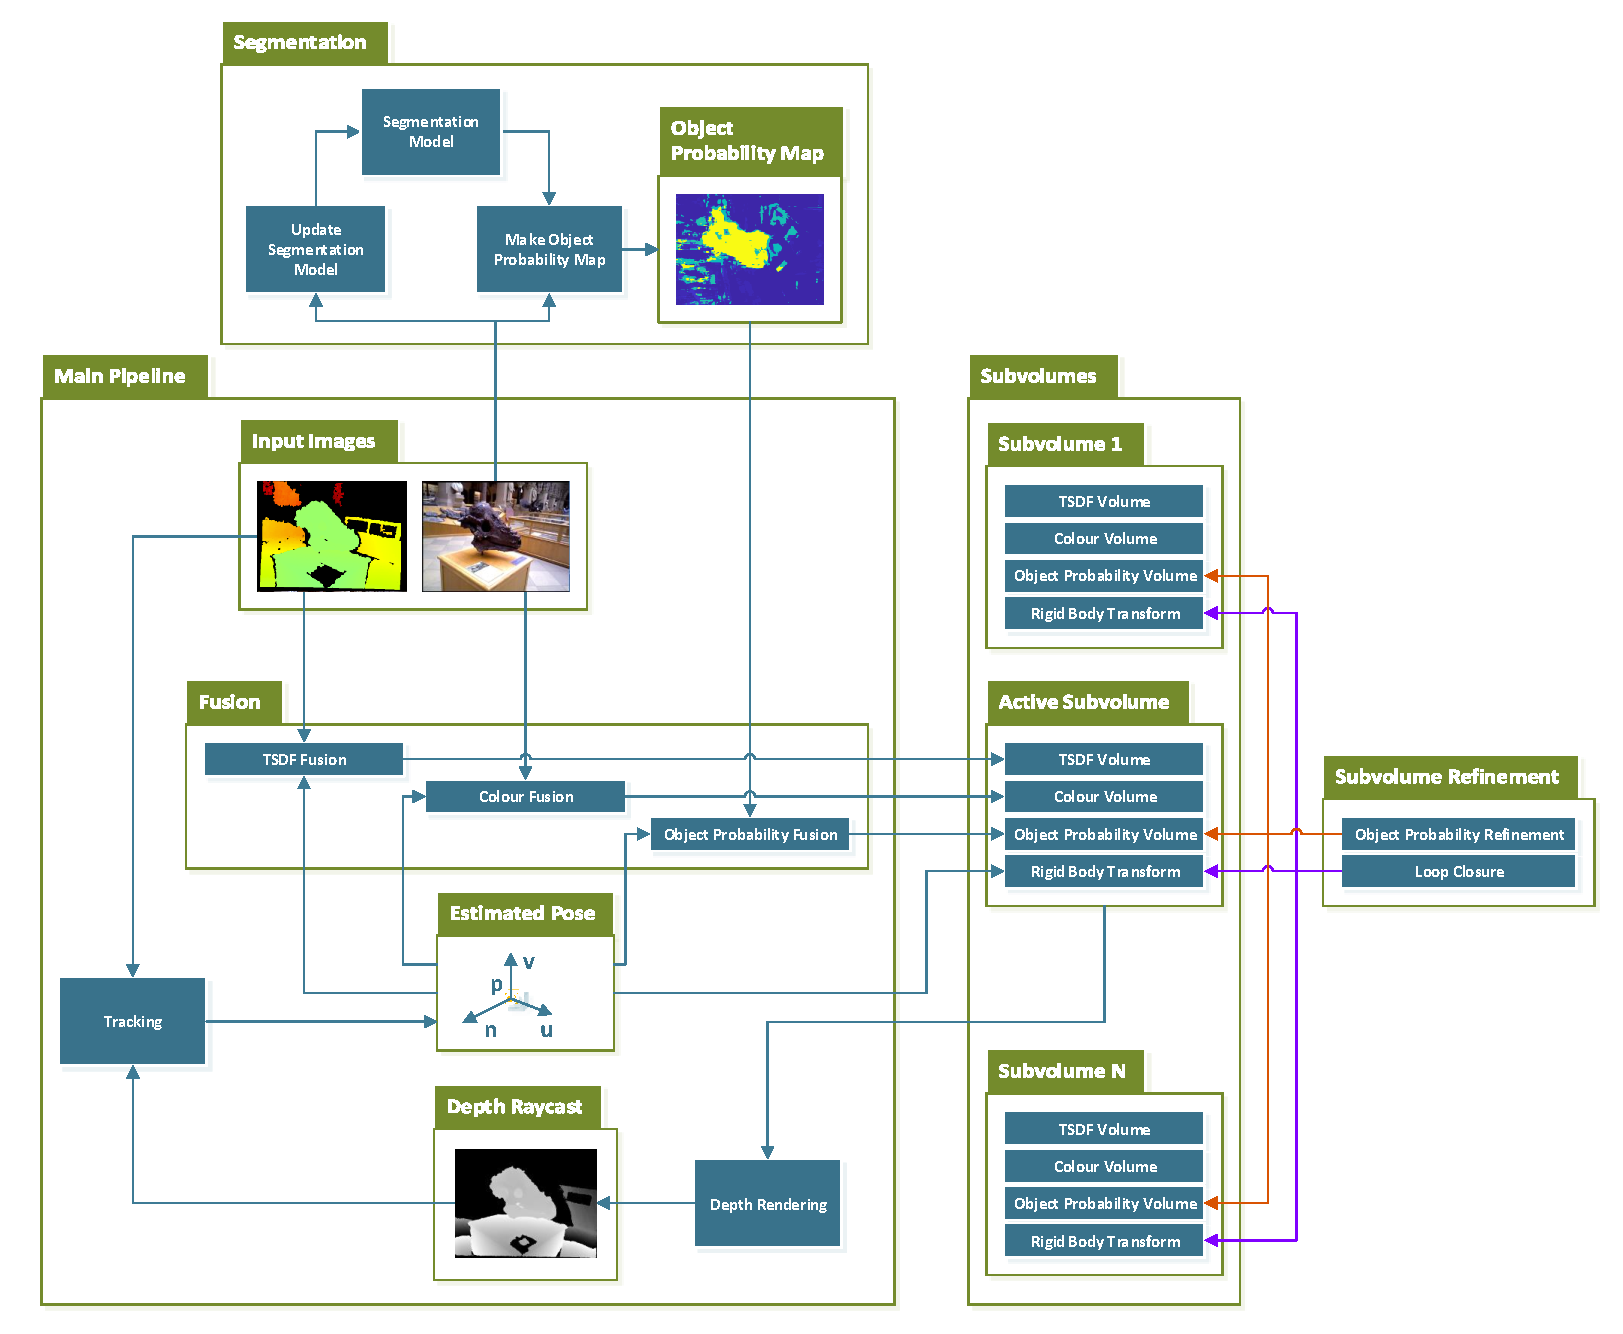
\includegraphics[width=\linewidth]{figures/object_recon/pipeline.pdf}
  \caption[Probabilistic Object Reconstruction Pipeline]
  {The pipeline of the proposed Object Reconstruction approach.}
\end{figure}

\section{Probabilistic Formulation of Object Reconstruction}
\label{sec:probobj_prob_formulation}
The surface map and camera pose are estimated using the standard KinectFusion
like pipeline of \cite{Newcombe2011,Prisacariu2014}. The surface is represented
as the Zero Level Set of a TSDF discretised over voxels, with the isosurface 
embedding built by a weigted mean of new observations, as outlined in Equations
\ref{eqn:sdf_update} and \ref{eqn:sdf_weight_update}. Camera pose estimation is
performed with ICP, as outlined in Section \ref{subsec:moseg_static_camera_trackin} 
and is run quasi-simultaneously against the evolving map. Here, inspired by 
\cite{Kolev2006}, this procedure is augmented by estimating the posterior probability, 
per map voxel, of belonging to the object of interest. This volume of posterior 
probabilities is updated at each time step, in parallel to the fusion process in the 
mapping and pose estimation components of the pipeline. The representation of the 
reconstructed object comprises multiple ``subvolumes'', each pertaining to some 
patch on the object surface. New subvolumes are created when sufficiently many new 
voxels have been allocated and have had SDF data integrated. By ensuring overlap
between the subvolumes, transformations between them can be found and pose
inconsistencies addressed, online. Empirically, the threshold for starting a new
subvolume is defined as the event when $50\%$ of the voxels fused in to the
current volume are newly observed points, such that there is sufficient overlap 
between two subvolumes that shall later be registered.

\subsection{Volumetric Appearance Model}
\label{subsec:probobj_vol_appearance_model}
At each observed RGBD frame, the object posterior probabilities for the visible
voxels in the active subvolume are updated via an appearance-derived probability
map for that frame. Under the assumption of conditional independence between
frames (for sake of tractability), the posterior probability of a given voxel
$\psi \in \Psi$ belonging to the object has the following form(noting that
$\Phi \subset \Psi$):
\begin{equation}
\label{eqn:probobj_voxel_posterior}
P(\psi \in \Phi | \Omega, p) = \prod_{t=0}^{\infty}
P(\psi_{t} \in \Phi | \Omega_{t}, p_{t})
\end{equation}
where $\Psi$ is the volume of voxels for which measurements are accumulated,
$\Phi$  is the volume of voxels pertaining to the object $\mathbf{\Phi}$ of 
interest, $\Omega_{t}$ is the current RGBD image observation at time $t$ and 
$p_{t}$ is the currently tracked pose at time $t$. Equation 
\ref{eqn:probobj_voxel_posterior} encodes the probability of a voxel belonging 
to the object of interest as the product of instantaneous appearance-derived 
pixel-wise conditionals. Note that in the above, $\Phi$ is a discretisation of 
the continuous $\Phi$ in the probabilistic formulation that follows.

\subsection{Full Joint Definition}
\label{subsec:probobj_full_joint}
Central to the proposed system is the aforementioned volume of appearance based
posterior probabilities pertaining to a voxel wise membership of either the
object voxel set or the non object (background) voxel set. This allows
formulation of the full joint distribution over the object as the Probabilistic
Graphical Model (PGM) of Figure \ref{fig:probobj_pgm1}.
\begin{figure}[h]
  \label{fig:probobj_pgm1}
  \centering
  \resizebox {0.4\linewidth}{!}{
    \begin{tikzpicture}
      % Declare nodes.
      \node[latent] (phi) {$\Phi$};
      \node[latent, right=of phi] (u) {$u$};
      \node[latent, below=of u] (L) {$L$};
      \node[obs, right=of u, yshift=-1cm] (omega) {$\Omega$};
      \node[obs, right=of u, yshift=1cm] (p) {$p$};
      
      % Setup plates.
      \plate[inner sep=0.25cm] {plate1} {(omega) (p)} {t, p};
      \plate[inner sep=0.25cm] {plate2} {(u) (phi)} {$\Psi$};
      \plate[inner sep=0.25cm] {plate3} {(L)} {s, s'};
      
      % Setup edges.
      \edge {omega, p} {u, L}
      \edge {L} {phi}
      \edge {u} {phi}
    \end{tikzpicture}
  }
  \caption[Probabilistic Object Reconstruction Formulation I]
  {Probabilistic Graphical Model representing the full Joint
    Distribution over the shape $\mathbf{\Phi}$ of the object of interest.}
\end{figure}

Where $\Phi$ is the shape of the object to be reconstructed (represented as a
subset of voxels for which surface data has been integrated into the relevant
TSDF), $u$ is the appearance model volume (aforementioned appearance Posteriors 
of Equation \ref{eqn:probobj_voxel_posterior}), $L$ is the set of consistency 
constraints for each adjacent sub volume pair in the form of rigid body 
transformations, $\Omega$ is the set of RGBD image pixels and $p$ the set of 
poses over time.

The PGM given in Figure \ref{fig:probobj_pgm1} leads to the following
factorisation over the full Joint Distribution.
\begin{equation}
  \label{eqn:probobj_full_joint}
  P(\Phi, \Omega, p, u, L) = 
  \prod_{\psi \in \Psi}\prod_{s, s' \in \mathcal{S}}
  P(\Phi \given u_{\psi}, L_{s, s'}) 
  \prod_{t=0}^{\infty}\prod_{p \in \mathcal{P}}
  P(u_{\psi} \given \Omega_{p, t}, p_{t})
  P(L_{s, s'} \given \Omega_{p, t}, p_{t})
  P(L_{s, s'})P(p_{t})P(\Omega_{p, t})
\end{equation}
Where in Equation \ref{eqn:probobj_full_joint}, $\Psi$ is the set of voxels
across all subvolumes, $\mathcal{P}$ is the set of RGBD pixels for a given 
frame $\Omega_{t}$ and $\mathcal{S}$ is the set of subvolumes. Note that the 
notation $s, s' \in \mathcal{S}$ refers to pairs of adjacent, overlapping 
subvolumes.

If pixel-wise independence is assumed in the RGBD observations and temporal
independence is assumed in the poses, the plate containing $\Omega$ and $p$ can
be removed as shown in Figure \ref{fig:probobj_pgm2}.
\begin{figure}[h]
  \label{fig:probobj_pgm2}
  \centering
  \resizebox {0.4\linewidth}{!}{
    \begin{tikzpicture}
      % Declare nodes.
      \node[latent] (phi) {$\Phi$};
      \node[latent, right=of phi] (u) {$u$};
      \node[latent, below=of u] (L) {$L$};
      \node[obs, right=of u, yshift=-1cm] (omega) {$\Omega$};
      \node[obs, right=of u, yshift=1cm] (p) {$p$};
      
      % Setup plates.
      \plate[inner sep=0.25cm] {plate3} {(L)} {s, s'};
      \plate[inner sep=0.25cm] {plate2} {(u) (phi)} {$\Psi$};
      
      % Setup edges.
      \edge {omega, p} {u, L}
      \edge {L} {phi}
      \edge {u} {phi}
    \end{tikzpicture}
  }
  \caption[Probabilistic Object Reconstruction Formulation II]
  {Probabilistic Graphical Model representing the simplified Joint
    Distribution over the shape $\mathbf{\Phi}$ of the object of interest.}
\end{figure}

The simplifications transforming the PGM of Figure \ref{fig:probobj_pgm1} in to
that of Figure \ref{fig:probobj_pgm2} lead to the following factorisation of the
Joint Distribution over $\mathbf{\Phi}$.
\begin{equation}
  \label{eqn:probobj_simplified_joint}
  P(\Phi, \Omega, p, u, L) = 
  \prod_{\psi \in \mathbf{\Psi}}P(\Phi \given u_{\psi})
  \prod_{s, s' \in \mathcal{S}}P(u_{\psi} \given \Omega, p, L_{s, s'})
  P(L_{s, s'} \given \Omega, p) P(L_{s, s'})P(p)P(\Omega)
\end{equation}

The formalisms defined in Figures \ref{fig:probobj_pgm1} and
\ref{fig:probobj_pgm2} and Equations \ref{eqn:probobj_full_joint} and
\ref{eqn:probobj_simplified_joint} describe a probabilistic framework in which
online corrections can be made to the reconstructed model (piecewise over
subvolumes) to counter errors caused by pose tracking inconsistencies. As with
scene scale dense SLAM systems \cite{Newcombe2011, Prisacariu2014, NieBner2013},
the presented system follows a pipeline that consists of a tracking stage and an
integration stage, as outlined in Section \ref{sec:moseg_static_fusion}.

However, the presented formulation of this pipeline consists of an
additional, novel estimation module that relies on the use of a subvolume
representation to correct tracking errors by applying rigid body transformations
to the subsegments of the reconstructed shape (the subvolumes) to correct their
alignment when there are intra subsegment tracking inconsistencies. As inference
on the Joint Distribution of the presented probabilistic model is intractable, 
conditional independence assumptions are made that empirically do not appear to 
cause any functional issues. 

Note that only voxels whose appearance posterior is greater for the foreground 
class are used in the correction procedure; only voxels that satisfy the probabilistic 
condition $P(\psi \in \Phi | \Omega, p) > 1 - P(\psi \in \Phi | \Omega, p)$ are 
considered.

\subsection{Appearance Marginal}
Continuing on from the formulation given in Equation \ref{eqn:probobj_simplified_joint}, 
the appearance model $u$ may be marginalised as follows.
\begin{align}
  \label{eqn:probobj_appearance_marginal}
  % Line 1.
  P(\Phi, \Omega, p, L) & =
  \int_{-\infty}^{\infty} \Bigg[ 
  \prod_{\psi \in \mathbf{\Psi}} P(\Phi \given u_{\psi})
  \prod_{s, s' \in \mathcal{S}}P(u_{\psi} \given \Omega, p, L_{s, s'})
  P(L_{s, s'} \given \Omega, p) P(L_{s, s'})P(p)P(\Omega) \Bigg] \intd{u} \\
  % Line 2.
  & = \prod_{\psi \in \mathbf{\Psi}} 
  \int_{-\infty}^{\infty} \Bigg[ P(\Phi \given u_{\psi})
  \prod_{s, s' \in \mathcal{S}}P(u_{\psi} \given \Omega, p, L_{s, s'})
  P(L_{s, s'} \given \Omega, p) P(L_{s, s'})P(p)P(\Omega) \Bigg] \intd{u} \\
  & = \prod_{s, s' \in \mathcal{S}} P(L_{s, s'} \given \Omega, p)
  P(L_{s, s'})P(p)P(\Omega)P(\mathbf{\Phi})
\end{align}
Note that the Appearance Posterior Volume outlined in Section 
\ref{subsec:probobj_vol_appearance_model} is reintroduced later in this work in
Section \ref{} for the purposes of subvolume alignment and determining the
subset of voxels $\mathbf{\Phi} \subset \mathbf{\Psi}$ that determine the target
object shape.

Further details pertaining to the inference procedure for the per-subvolume
deformations is provided in Section \ref{sec:probobj_model_correction}.

\section{Online Model Correction}
\label{sec:probobj_model_correction}
The tracking consistency constraints denoted by the variables $L_{s, s'}$ such
that $s, s' \in \mathcal{S}$ with $\mathcal{S}$ being the set of overlapping
subvolume pairs $s, s'$ in the Probabilistic Graphical Models given by Figures
\ref{fig:probobj_pgm1} and \ref{fig:probobj_pgm2} can be enforced in terms of
minimising the disparity between each pair of adjacent subvolumes. The effect of
this minimsation being that consistency in the pose estimation phase of the
pipeline outlined in Figure \ref{fig:probobj_pipeline_diagram} is enforced. The
objective of this procedure is to infer a robust and consistent deformation
transformation for the subvolume pair.

\subsection{Alignment MAP Estimate}
\label{subsec:probobj_alignment_map}
Referring back to the joint distribution of Equation \ref{eqn:probobj_simplified_joint}, 
to achieve the aforementioned minimisation of disparity between overlapping subvolumes, 
a Maximum a Posteriori (MAP) estimate is desirable. As such, a MAP estimate over $L_{s, s'}$ 
in Equation \ref{eqn:probobj_simplified_joint} for a given subvolume pair $s, s'$ may be
derived as follows.
\begin{align}
  \label{eqn:probobj_map_estimate}
  % Line 1.
  P(\Omega, p | L_{s, s'}) & \propto \prod_{s, s' \in \mathcal{S}}
  \frac{P(L_{s, s'} | \Omega, p) 
  P(\Omega | p)P(p)P(L_{s, s'})}
  {\displaystyle\int_{-\infty}^{\infty} P(L_{s, s'} \given \Omega, p)
  \intd{L_{s, s'}}} P(\Phi) \\
  % Line 2.
  & \propto \prod_{s, s' \in \mathcal{S}} P(L_{s, s'} | \Omega, p) P(\Omega | p)
  P(p)P(L_{s, s'})P(\Phi) \\
  % Line 3.
  & \propto \prod_{s, s' \in \mathcal{S}} P(L_{s, s'} | \Omega, p)P(L_{s, s'})
  P(\Phi)
\end{align}
Note that in the third step of Equation \ref{eqn:probobj_map_estimate} the
distributions $P(\Omega | p)$ and $P(p)$ are taken to be uniform and as such may
be omitted whilst retaining proportionality. The prior distribution $P(L_{s, s'})$ is
conjugate to $P(L_{s, s'} | \Omega, p)$ and is of the form of a Multivariate
Gaussian Distribution $\mathcal{N}(\mathbf{0} \given \mathbf{I})$ over the
$\mathbb{SE}(3)$ deformation parameters described in Section 
\ref{subsub:moseg_static_camera_attitude}. The choice of such a prior distribution
is motivated by the assumption that motion between consecutive frames is minor,
thus the given prior will have the effect of constraining the $\mathbb{SE}(3)$
transformation as such. The prior distribution $P(\Phi)$ serves as a
\textit{Surface Prior} to mitigate the effect of noise introduced in to the TSDF
volumes. The form of $P(\Phi)$ shall be discussed in Section
\ref{subsec:probobj_analytic_alignment_map}.

The rationale of Equation \ref{eqn:probobj_map_estimate} is that the deformation
$L_{s, s'}$ applied to the subvolume $s$ maximises the posterior probability of
observing the current pose $p$ given the current RGBD frame $\Omega$ by reducing
the variance of the result of the pose estimation phase of the pipeline. As such,
global tracking variance (quantified by the proportion of outliers in the result
of the ICP component of the pipeline) is reduced by enforcing local consistency,
also improving global consistency and thus the quality of the resultant
reconstruction.

\subsection{Analytic Form of Alignment MAP Estimate}
\label{subsec:probobj_analytic_alignment_map}
With the probabilistic framework now outlined, the analytic form of the
posterior given in Equation \ref{eqn:probobj_map_estimate} may be explored. The
likelihood term in Equation \ref{eqn:probobj_map_estimate} quantifies the
ability of the constraint $L_{s, s'}$ to maximise consistency between subvolumes
$s$ and $s'$, with respect to observed RGBD frame $\Omega$ and pose $p$. By
quantifying the likelihood only for voxels in $s$ and $s'$ that are visible in
the current view frustrum at time $t$, the posterior $P(\Omega, p | L_{s, s'})$
is given. As outlined in Section \ref{subsec:probobj_alignment_map}, the prior
on the constraints $L_{s, s'}$ has the form of a Multivariate Gaussian
Distribution of the form $\mathcal{N}(\mathbf{0}, \mathbf{I})$.

As such, the analytic form of the likelihood term $P(L_{s, s'} | \Omega, p)$ is
given as follows.
\begin{equation}
  \label{eqn:probobj_likelihood_analytic}
  P(L_{s, s'} | \Omega, p) = \prod_{(s, s') \in \mathcal{S}}
  \frac{1}{\sqrt{2 \pi \sigma}}
  \exp{\frac{-\Big[\Phi_{s}\Big(\mathbf{x}\Big) -
  \Phi_{s'}\Big(\Lambda(\mathbf{x}, \mathbf{p}, \mathbf{t})\Big)\Big]^{2}}
  {2\sigma^{2}}}
\end{equation}

In Equation \ref{eqn:probobj_likelihood_analytic}, the function $\Lambda(.)$
applies the resultant $\mathbb{SE}(3)$ transform to a given voxel position
$\mathbf{x}$ and is defined as follows.
\begin{align}
  \label{eqn:probobj_lambda_fn}
  \Lambda(\mathbf{x}, \mathbf{p}, \mathbf{t}) &=
  \mathbf{R}_{\mathbf{p}} \mathbf{x} + \mathbf{t}\\
  &= 
  \begin{bmatrix}
    \mathbf{R}_{\mathbf{p}} & \mathbf{t} \\
    \mathbf{0} & 1
  \end{bmatrix}
  \mathbf{x}
\end{align}
In Equation \ref{eqn:probobj_lambda_fn} $R_{\mathbf{p}}$ is the $\mathbb{SO}(3)$
rotation matrix generated from the Rodrigues parameters given by the Vector
$\mathbf{p}$. Recall the definition of the Rodrigues paramaterisation given in
Equation \ref{eqn:rodriguez_matrix_eq} of Section
\ref{subsub:moseg_static_camera_attitude}.

The form of the aforementioned surface prior $P(\Phi)$ is taken to be that of
the Logistic Distribution, due to the ``symmetric'' $1 - f(x) = f(-x)$
and ``squashing'' $\texttt{Range}[f(x)] = [0, 1]$ properties of it's Cumulative
Density Function (CDF). The PDF of the Logistic Distribution is given as follows.
\begin{equation}
  \label{eqn:probobj_logistic_dist}
  \text{Logistic}(x \given \mu, \sigma) = \frac
  {e^{-\frac{x - \mu}{\sigma}}}
  {\sigma \big( 1 + e^{-\frac{x - \mu}{\sigma}} \big)^{2}}
\end{equation}

To encode the probability of a given voxel $\psi \in \mathbf{\Psi}$ encoding an
isosurface point, represented as the Zero Level Set defined in Equation
\ref{eqn:zero_level_definition} of a TSDF, it is desirable to quantify the
probability with a function that has the aforementioned properties. As such, the
CDF of $P(\Phi)$ is derived as follows.
\begin{align}
  \label{eqn:probobj_surface_prior_cdf}
  % Line 1.
  %P(\Phi < b) &= \int_{-\infty}^{b} \text{Logistic}
  %(\Phi \given \mu, \sigma) \intd{\Phi}\\
  % Line 2.
  \bar{P}(\Phi) &\propto P(\Phi < b)\\
  &\propto \int_{-\infty}^{b} \frac
  {e^{-\frac{\Phi - \mu}{\sigma}}}
  {\sigma \Big( 1 + e^{-\frac{\Phi - \mu}{\sigma}} \Big)^{2}} \intd{\Phi}\\
  % Line 3.
  &\propto \lim_{y\to -\infty} \int_{y}^{b} \frac
  {e^{\frac{-\Phi + \mu}{\sigma}}}
  {\sigma \Big( 1 + e^{\frac{-\Phi + \mu}{\sigma}} \Big)^{2}} \intd{\Phi}\\
  % Line 4.
  &\propto \lim_{y\to -\infty} \frac{1}{\sigma} \int_{y}^{b}
  \frac{e^{\frac{u}{s}}}{\Big( 1 + e^{\frac{u}{\sigma}} \Big)^{2}} \intd{u}\\
  \shortintertext{Where $u = -\Phi + \mu$ and $\intd{u} = -\intd{\Phi}$}
  % Line 5.
  &\propto \lim_{y\to -\infty} -\int_{y}^{b}
  \frac{e^{p}}{\Big( 1 + e^{p} \Big)^{2}} \intd{p}\\
  \shortintertext{Where $p = \frac{u}{\sigma}$ and $\intd{p} = \frac{1}{\sigma}
  \intd{u}$}
  % Line 6.
  &\propto \lim_{y\to -\infty} -\int_{y}^{b} \frac{1}{w^{2}} \intd{w}\\
  \shortintertext{Where $w = 1 + e^{p}$ and $\intd{w} = e^{p} \intd{p}$}
  % Line 7.
  &\propto \lim_{y\to -\infty} \Bigg[ \frac{1}{w} + C \Bigg]_{y}^{b}\\
  % Line 8.
  &\propto \lim_{y\to -\infty} \Bigg[ \frac{1}{1 + e^{p}} + C \Bigg]_{y}^{b}\\
  % Line 9.
  &= \lim_{y\to -\infty} \Bigg[ \frac{1}{1 +e^{\frac{u}{\sigma}}} + C
  \Bigg]_{y}^{b}\\
  % Line 10.
  &\propto \lim_{y\to -\infty} \Bigg[ \frac{1}{1 + e^{\frac{-\Phi + \mu}{\sigma}}} +
  C \Bigg]_{y}^{b}\\
  &\propto \Bigg[ \frac{1}{1 + e^{\frac{-\Phi + \mu}{\sigma}}} + C \Bigg]_{\Phi = b}
  - \Bigg[ \left. \lim_{y\to -\infty} \frac{1}{1 + e^{\frac{-\Phi + \mu}{\sigma}}}
  \right\rvert_{\Phi = y} + C \Bigg]\\
  &\propto \frac{1}{1 + e^{\frac{-\Phi + \mu}{\sigma}}}
\end{align}
Given the Cumulative Density Function derived in Equation
\ref{eqn:probobj_surface_prior_cdf}, the prior $P(\Phi)$ is defined as follows.
\begin{align}
  \label{eqn:probobj_surface_prior}
  \bar{P}(\Phi) &\propto \left. \int_{-\infty}^{b} \frac
  {e^{-\frac{\Phi - \mu}{\sigma}}}
  {\sigma \Big( 1 + e^{-\frac{\Phi - \mu}{\sigma}} \Big)^{2}} \intd{\Phi}
  \right\rvert_{\mu = 0, \sigma = 1}\\
  &\propto \frac{1}{1 + e^{-\Phi}}
\end{align}
It is evident from Equation \ref{eqn:probobj_surface_prior} that under an 
appropriate paramaterisation, the CDF of the Logistic Distribution is the 
Logistic Sigmoid function prevelant in the Artificial Neural Network literature. 
As given in Equation \ref{eqn:probobj_surface_prior} the mean $\mu$ and standard 
deviation $\sigma$ are $0$ and $1$, respectively.

Finally, the analytic form of the log-posterior is given as follows, optimising
for the Rodrigues parameters $p$ and translation vector $t$ of the constraint
$L_{s, s'}$ between subvolumes $s$ and $s'$.
\begin{align}
  \label{eqn:probobj_log_posterior}
  % Line 1.
  \ln P(\Omega, p | L_{s, s'}) &\propto \ln
  \prod_{s, s' \in \mathcal{s}} P(L_{s, s'} | \Omega, p)P(L_{s, s'})\bar{P}(\Phi)\\
  % Line 2.
  &\propto \sum_{s, s' \in \mathcal{S}} \ln P(L_{s, s'} | \Omega, p) +
  \sum_{s, s' \in \mathcal{S}} \ln P(L_{s, s'}) +
  \sum_{s, s' \in \mathcal{S}} \ln \bar{P}(\Phi)\\
  % Line 3.
  &\propto \sum_{s, s' \in \mathcal{S}} \Bigg[\ln \frac{1}{\sqrt{2 \pi \sigma}}
  \exp{\frac{-\Big[\Phi_{s}\big(\mathbf{x}\big) - \Phi_{s'}
  \big(\Lambda(\mathbf{x}, \mathbf{p}, \mathbf{t})\big)\Big]^{2}}
  {2\sigma^{2}}} \\
  &\phantom{\propto \sum_{s, s' \in \mathcal{S}} \Bigg[} % SPLIT LINE
  + \ln \frac{-\frac{1}{2} e^{\mathbf{p}^{T}\mathbf{\Sigma}^{-1}\mathbf{p}}}
  {\sqrt{(2\pi)^{k}\left|\mathbf{\Sigma}\right|}} +
  \ln \frac{1}{1 + e^{-\Phi}}\Bigg]\\
  % Line 4.
  &\propto \sum_{s, s' \in \mathcal{S}} \Bigg[ -\ln(2\pi\sigma) -
  \frac{\Big[\Phi_{s}\big(\mathbf{x}\big) -
  \Phi_{s'}\big(\Lambda(\mathbf{x}, \mathbf{p}, \mathbf{t})\big)\Big]^{2}}{2\sigma^{2}} -
  \frac{1}{2} \ln \left|\mathbf{\Sigma}\right|\\ 
  &\phantom{\propto \sum_{s, s' \in \mathcal{S}} \Bigg[} % SPLIT LINE
  - \frac{1}{2} \mathbf{p}^{T}\mathbf{\Sigma}^{-1}\mathbf{p} -
  \ln(1 + e^{-\Phi}) \Bigg]\\
  % Line 5.
  &\propto \sum_{s, s' \in \mathcal{S}} \Bigg[ -\ln(2\pi\sigma) -
  \frac{\Big[\Phi_{s}(\mathbf{x}) -
  \Phi_{s'}\big(\Lambda(\mathbf{x}, \mathbf{p}, \mathbf{t})\big)\Big]^{2}}{2\sigma^{2}} -
  \frac{1}{2} \mathbf{p}^{T}\mathbf{p} \\
  &\phantom{\propto \sum_{s, s' \in \mathcal{S}} \Bigg[} % SPLIT LINE
  - \ln(1 + e^{-\Phi}) \Bigg]
\end{align}

As with the gradients derived in Section \ref{subsec:moseg_static_camera_tracking}, the 
gradient update when optimising Equation \ref{eqn:probobj_log_posterior} takes the familiar 
Levenberg-Marquardt update form, akin to that of Equation \ref{eqn:lm_update}.

\subsection{Optimisation for MAP Inference}
\label{subsec:probobj_map_optimisation}
To infer the optimal consistency constraints between adjacent subvolumes, the
log-posterior given in Equation \ref{eqn:probobj_log_posterior} may be optimised
using second order gradient based methods such as Levenberg-Marquardt. As with
the ICP procedure outlined in Section \ref{subsub:moseg_static_camera_poserec},
the optimisation is performed with respect to the three Rodrigues rotation
parameters $\alpha$, $\beta$, $\gamma$ and translation parameters $t_{x}$,
$t_{y}$ and $t_{z}$ of the target $\mathbb{SE}(3)$ transformation.

In a similar manner to the process outlined in Section
\ref{subsub:moseg_static_camera_poserec}, the target energy function must be
differentiated with respect to each of the $\mathbb{SE}(3)$ parameters. In this
case, the log-posterior of Equation \ref{eqn:probobj_log_posterior} is the
target energy function and shall be denoted $E(.)$ in the following derivation.
The derivation of the partial derivatives of $E(.)$ with respect
to the Rodrigues rotational parameters is as follows for some parameter
$\tau \in \{\alpha, \beta, \gamma\}$.
\begin{align}
  \label{eqn:probobj_log_post_rot_grad}
  % Line 1.
  \frac{\partial E}{\partial \tau} &=
  \sum_{s, s' \in \mathcal{S}} \Bigg[ - \frac{\partial}{\partial \tau}
  \ln(2\pi\sigma) - \frac{\partial}{\partial \tau}
  \frac{\Big[\Phi_{s}\big(\mathbf{x}\big) -
  \Phi_{s'}\big(\Lambda(\mathbf{x})\big)\Big]^{2}}{2\sigma^{2}} -
  \frac{\partial}{\partial \tau} \frac{1}{2} \mathbf{p}^{T}\mathbf{p} -
  \frac{\partial}{\partial \tau} \ln(1 + e^{-\Phi})
  \Bigg]\\
  % Line 2.
  &= \sum_{s, s' \in \mathcal{S}} \Bigg[ \frac{1}{2\sigma^{2}}
  \frac{\partial}{\partial \tau}
  \Big[\Phi_{s}\big(\mathbf{x}\big) - \Phi_{s'}\big(\Lambda(\mathbf{x})\big)\Big]^{2} -
  \frac{1}{2} \frac{\partial}{\partial \tau}
  \mathbf{p}^{T}\mathbf{p} - \frac{\partial}{\partial \tau} \ln(1 + e^{-\Phi})
  \Bigg]\\
  % Line 3.
  &= \sum_{s, s' \in \mathcal{S}} \Bigg[ \frac{1}{2\sigma^{2}}
  \frac{\partial \phi}{\partial \Phi} \frac{\partial \Phi}{\partial \Lambda}
  \frac{\partial \Lambda}{\partial \mathbf{R}_{\tau}} -
  \frac{1}{2} \frac{\partial}{\partial \tau}
  \mathbf{p}^{T}\mathbf{p} - \frac{\partial}{\partial \tau} \ln(1 + e^{-\Phi})
  \Bigg]\\
  \shortintertext{Where $\phi(.) =
  \big(\Phi_{s}(\mathbf{x}) - \Phi_{s'}(\Lambda(\mathbf{x}))\big)^{2}$}
  % Line 4.
  &= \sum_{s, s' \in \mathcal{S}} \Bigg[ \sigma^{2} \phi(.)
  \frac{\partial \Phi}{\partial \Lambda}
  \frac{\partial \Lambda}{\partial \mathbf{R}_{\tau}} -
  \frac{1}{2} \frac{\partial}{\partial \tau}
  \mathbf{p}^{T}\mathbf{p} - \frac{\partial}{\partial \tau} \ln(1 + e^{-\Phi})
  \Bigg]\\
  % Line 5.
  &= \sum_{s, s' \in \mathcal{S}} \Bigg[ \sigma^{2} \phi(.)
  \frac{\partial \Phi}{\partial \Lambda}
  \frac{\partial \Lambda}{\partial \mathbf{R}_{\tau}} - \mathbf{p}^{T} -
  \frac{\partial}{\partial \tau} \ln(1 + e^{-\Phi})
    \Bigg]\\
  % Line 6.
  &= \sum_{s, s' \in \mathcal{S}} \Bigg[ \sigma^{2} \phi(.)
  \frac{\partial \Phi}{\partial \Lambda}
  \frac{\partial \Lambda}{\partial \mathbf{R}_{\tau}} - \mathbf{p}^{T} +
  \frac{1}{1 + e^{\Phi}} \frac{\partial \Phi}{\partial \Lambda}
  \frac{\partial \Lambda}{\partial \mathbf{R}_{\tau}} \Bigg]
\end{align}

\section{Volumetric Segmentation and Explicit Loop Closure Detection}
The final component of the proposed pipeline performs a segmentation in three
dimensional observed model space to perform refinements over the appearance
posteriors that separate the voxels pertaining to the object of interest from
those that have irrelevant measurements integrated, i.e. background measurements
that have not been used to perform pose estimation and as such have not been rendered.

This segmentation is formulated within a CRF framework, with each node in the
CRF graph representing a set of neighbouring voxels in space, where connections
are made between adjacent voxel neighbourhoods. This segmentation process is
posed as an energy minimisation problem to optimise for a cut in downsampled
voxel space between observations pertaining to the object of interest and those,
of irrelevant observations, such that a segmentation in 3D is obtained. The
central purpose of this segmentation is to refine the resultant output model of
the proposed object reconstruction system. The described CRF model is depicted
in Figure \ref{fig:probobj_crf}

\begin{figure}[h]
  \label{fig:probobj_crf}
  \centering
  \resizebox {0.5\linewidth}{!}{
    \begin{tikzpicture}[every node/.style={minimum size=1cm},on grid]
      % Define dimension and multiplier - tweakable.
      \newcommand\graphdim{2}
      \newcommand\multiplier{2}
      \newcommand\srad{0.8}

      % Define highlight node.
      \pgfmathtruncatemacro\hx{2}
      \pgfmathtruncatemacro\hy{2}
      \pgfmathtruncatemacro\hz{0}

      % Truncated Graph boundary nodes.
      \pgfmathtruncatemacro\gmin{-1}
      \pgfmathtruncatemacro\gmax{\multiplier*\graphdim + 1}

      % Draw Edges.
      \begin{scope}%[rotate around x=5]
        \foreach \i in {0,...,\graphdim}{
          \foreach \j in {0,...,\graphdim}{
            \foreach \k in {0,...,\graphdim}{
              % Get truncated x, y, and z. 
              \pgfmathtruncatemacro\x{\multiplier*\i}
              \pgfmathtruncatemacro\y{\multiplier*\j}
              \pgfmathtruncatemacro\z{\multiplier*\k}

              % Get truncated neigh left, right, up, down, forward and backward.
              \pgfmathtruncatemacro\nl{\x-\multiplier}
              \pgfmathtruncatemacro\nr{\x+\multiplier}
              \pgfmathtruncatemacro\nu{\y+\multiplier}
              \pgfmathtruncatemacro\nd{\y-\multiplier}
              \pgfmathtruncatemacro\nf{\z+\multiplier}
              \pgfmathtruncatemacro\nb{\z-\multiplier}

              % Left Neighbour Edge.
              \ifnum\nl>\gmin
                \draw[color=gray, line width=0.5mm] (\x, \y, \z) -- (\nl, \y, \z);
              \fi

              % Right Neighbour Edge.
              \ifnum\nr<\gmax
                \draw[color=gray, line width=0.5mm] (\x, \y, \z) -- (\nr, \y, \z);
              \fi

              % Up Neighbour Edge.
              \ifnum\nu<\gmax
                \draw[color=gray, line width=0.5mm] (\x, \y, \z) -- (\x, \nu, \z);
              \fi

              % Down Neighbour Edge.
              \ifnum\nd>\gmin
                \draw[color=gray, line width=0.5mm] (\x, \y, \z) -- (\x, \nd, \z);
              \fi

              % Forward Neighbour Edge.
              \ifnum\nf<\gmax
                \draw[color=gray, line width=0.5mm] (\x, \y, \z) -- (\x, \y, \nf);
              \fi

              % Backward Neighbour Edge.
              \ifnum\nb>\gmin
                \draw[color=gray, line width=0.5mm] (\x, \y, \z) -- (\x, \y, \nb);
              \fi
            }
          }
        }
      \end{scope}

      % Draw Nodes.
      \begin{scope}%[rotate around x=5]
        \foreach \i in {0,...,\graphdim}{
          \foreach \j in {0,...,\graphdim}{
            \foreach \k in {0,...,\graphdim}{
              % Get truncated x, y and z.
              \pgfmathtruncatemacro\x{\multiplier*\i}
              \pgfmathtruncatemacro\y{\multiplier*\j}
              \pgfmathtruncatemacro\z{\multiplier*\k}

              % Scale hx, hy and hz.
              \pgfmathtruncatemacro\hhx{\multiplier*\hx}
              \pgfmathtruncatemacro\hhy{\multiplier*\hy}
              \pgfmathtruncatemacro\hhz{\multiplier*\hz}

              % Get truncated neigh left, right, up, down, forward and backward.
              \pgfmathtruncatemacro\hl{\hhx-\multiplier}
              \pgfmathtruncatemacro\hr{\hhx+\multiplier}
              \pgfmathtruncatemacro\hu{\hhy+\multiplier}
              \pgfmathtruncatemacro\hd{\hhy-\multiplier}
              \pgfmathtruncatemacro\hf{\hhz+\multiplier}
              \pgfmathtruncatemacro\hb{\hhz-\multiplier}

              % First colour as an ordinary node.
              \draw[color=blue!60] plot [mark=*, mark size=5] coordinates{(\x, \y, \z)}; 
              
              % If this is the node of interest.
              \pgfmathparse{\x==\hhx && \y==\hhy && \z==\hhz ? int(1) : int(0)}
              \ifnum\pgfmathresult>0
                \draw[color=green!50] plot [mark=*, mark size=5] coordinates{(\x, \y, \z)};
              \fi


              % If this is an x neighbour of the node of interest.
              \pgfmathparse{(\x==\hl || \x==\hr) && \y==\hhy && \z==\hhz ? int(1) : int(0)}
              \ifnum\pgfmathresult>0
                \draw[color=red!60] plot [mark=*, mark size=5] coordinates{(\x, \y, \z)};
              \fi

              % If this is an y neighbour of the node of interest.
              \pgfmathparse{(\y==\hu || \y==\hd) && \x==\hhx && \z==\hhz ? int(1) : int(0)}
              \ifnum\pgfmathresult>0
                \draw[color=red!60] plot [mark=*, mark size=5] coordinates{(\x, \y, \z)};
              \fi

              % If this is an y neighbour of the node of interest.
              \pgfmathparse{(\z==\hf || \z==\hb) && \x==\hhx && \y==\hhy ? int(1) : int(0)}
              \ifnum\pgfmathresult>0
                \draw[color=red!60] plot [mark=*, mark size=5] coordinates{(\x, \y, \z)};
              \fi
            }
          }
        }
      \end{scope}

      % Finally, draw the sphere of influence... Putin style!
      \begin{scope}
        % Scale hx, hy and hz.
        \pgfmathtruncatemacro\hhx{\multiplier*\hx}
        \pgfmathtruncatemacro\hhy{\multiplier*\hy}
        \pgfmathtruncatemacro\hhz{\multiplier*\hz}

        % Shade and draw the ball.
        \shade[ball color=green!60, opacity=0.3] (\hhx, \hhy, \hhz) circle (\srad cm);
      \end{scope}
    \end{tikzpicture}
  }
  \caption[3D CRF over Voxels]
  {The 3D CRF model over Voxel space.}
\end{figure}

The following energy function consists of the appearance posterior probabilities
accumulated during the on-line fusion process for a region in space as the
CRF unary potentials. The pairwise smoothing term represents the physical
appearance similarity of the observation regions represented by the
voxel neighbourhoods $\gamma$ and $\gamma^{'}$:
\begin{equation}
  \label{eqn:probobj_crf_energy}
  E_{n} = \prod_{t=0}^{\infty} \prod_{\psi \in \Psi_{n}}
  P(\psi \in \Phi \given \Omega_{t}, p_{t}) +
  P(\mathbb{E}[c]_{\gamma} \given \mathbb{E}[c]_{\gamma'})
\end{equation}

In Equation \ref{eqn:probobj_crf_energy} the terms $\mathbb{E}[c]_{\gamma}$ and
$\mathbb{E}[c]_{\gamma'}$ of the pairwise component of the energy function are
the expected values over appearance for the 3D regions $\gamma$ and $\gamma'$
respectively. Recall the unary term $P(\psi \in \Phi \given \Omega_{t}, p_{t})$
from Equation \ref{eqn:probobj_voxel_posterior} of Section
\ref{subsec:probobj_vol_appearance_model}.

In the implementation used in this work, the aforementioned cut in voxel space
is obtained by optimising the energy function of Equation \ref{eqn:probobj_crf_energy} 
within a Max-Flow framework \cite{BOYKOV} due to GPU parallelisation potential. However 
it should be noted that alternatives such as Variational Bayesian Mean Field approximations 
may also be of use \cite{KRAHENBUHL}.

\section{Qualitative Results}
\label{sec:probobj_qualitative}
Empirically the proposed system is capable of reconstructing a range of objects 
characterised by a range of different sizes and geometries. The experiments in 
this section demonstrate efficacy over the approach of \textit{Ren et al} 
\cite{Ren2013} for the task of obtaining closed, small object reconstructions 
from RGBD data. Each evaluation sequence is run on the system proposed in this 
chapter and through that of \textit{Ren et al}, with output snapshots taken at 
quarterly intervals for each sequence. In Section \ref{QUANT}, a Quantitative 
evaluation of Reconstruction quality is given.

\begin{figure}[h]
  \label{fig:probobj_rock_s3d}
  \centering
  \begin{tabular}{@{}c@{}}
    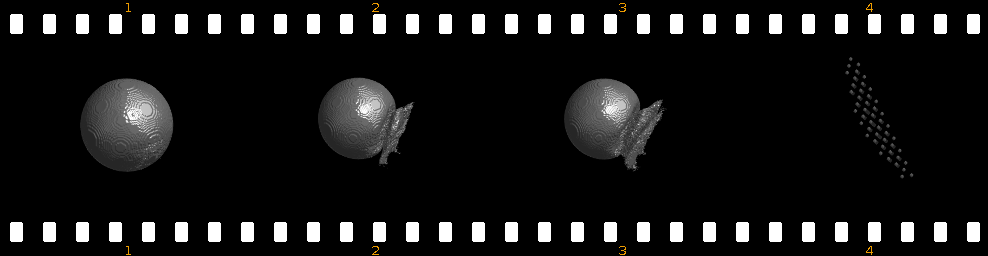
\includegraphics[width=.6\linewidth]{figures/object_recon/strips/rock_s3d.png} \\
    (a) \\
    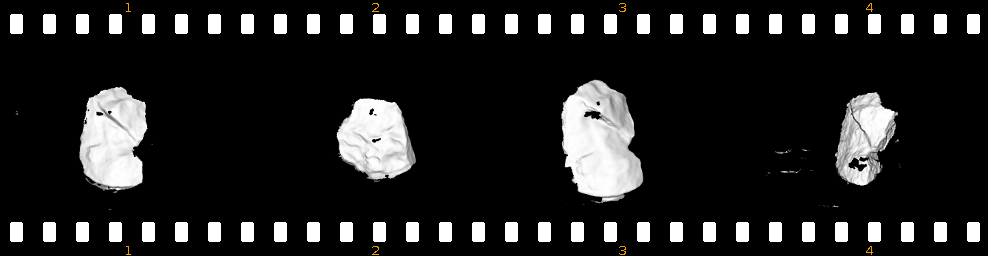
\includegraphics[width=.6\linewidth]{figures/object_recon/strips/rock.png} \\ 
    (b)\\
  \end{tabular}
  \caption[Probabilistic Object Reconstruction Qualitative Results I]
  {(a) The system of \textit{Ren et al} \cite{Ren2013} evolving a shape prior SDF 
  from RGBD observations on the Museum Rock sequence. (b) The proposed system reconstructing 
  the same object from observations of the Museum Rock sequence.}
\end{figure}

As can be observed in Figure \ref{fig:probobj_rock_s3d}, the proposed system of 
\textit{Ren et al} begins with a discretised SDF shape prior of a sphere that is 
evolved over time whilst simultaneously optimising for pose. However, it is evident 
that through the course of the sequence it is unable to evolve sufficiently to model 
the object of interest, contary to the approach outlined in this chapter.

\begin{figure}[h]
  \label{fig:probobj_dino_s3d}
  \centering
  \begin{tabular}{@{}c@{}}
    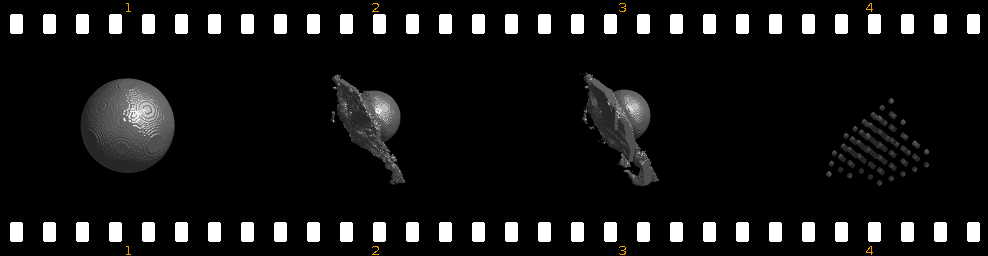
\includegraphics[width=.6\linewidth]{figures/object_recon/strips/dino_s3d.png} \\
    (a) \\
    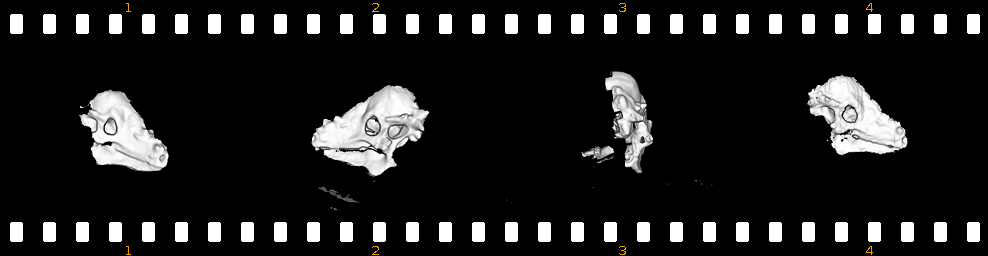
\includegraphics[width=.6\linewidth]{figures/object_recon/strips/dino.png} \\ 
    (b) \\
  \end{tabular}
  \caption[Probabilistic Object Reconstruction Qualitative Results II]
  {(a) The system of \textit{Ren et al} \cite{Ren2013} evolving a shape prior SDF 
  from RGBD observations on the Museum Dinosaur Head sequence. (b) The proposed system 
  reconstructing same the object from observations of the Museum Dinosaur Head sequence.}
\end{figure}

As with the example given in Figure \ref{fig:probobj_rock_s3d}, it can be seen in 
Figure \ref{fig:probobj_dino_s3d} that the system of \textit{Ren et al} is again 
unable to evolve the SDF shape prior suffiently to model the object of interest. As 
can be observed, again the proposed system of this work is capable of yielding a suitable 
reconstruction.

An additional evaluation is performed on the proposed systems ability to reconstruct 
a range of objects versus that of an implementation of the standard KinectFusion 
pipeline as outlined in Section \ref{MOSEG INTRO}. The central difference in the use 
of the two approaches for the purposes of this comparison is that in the proposed system, 
only the observed points of the live frame and of the reconstruction that belong to the 
object of interest are used for pose estimation. In the KinectFusion pipeline used 
as a base of comparison however, the entire scene is modelled as the camera is moved, 
with the reconstruction of the object of interest being segmented as a post processing 
step. As such, the results extracted from the KinectFusion pipeline are taken to be the 
ground truth reconstructions of the object of interest. This is due to the more robust 
pose estimation that would be expected from utilising all available geometric data 
for tracking, versus utilising only that of a single, potentially small object.

\begin{figure}[h]
  \label{fig:probobj_comp_itm}
  \centering
  \begin{tabular}{cccc}
    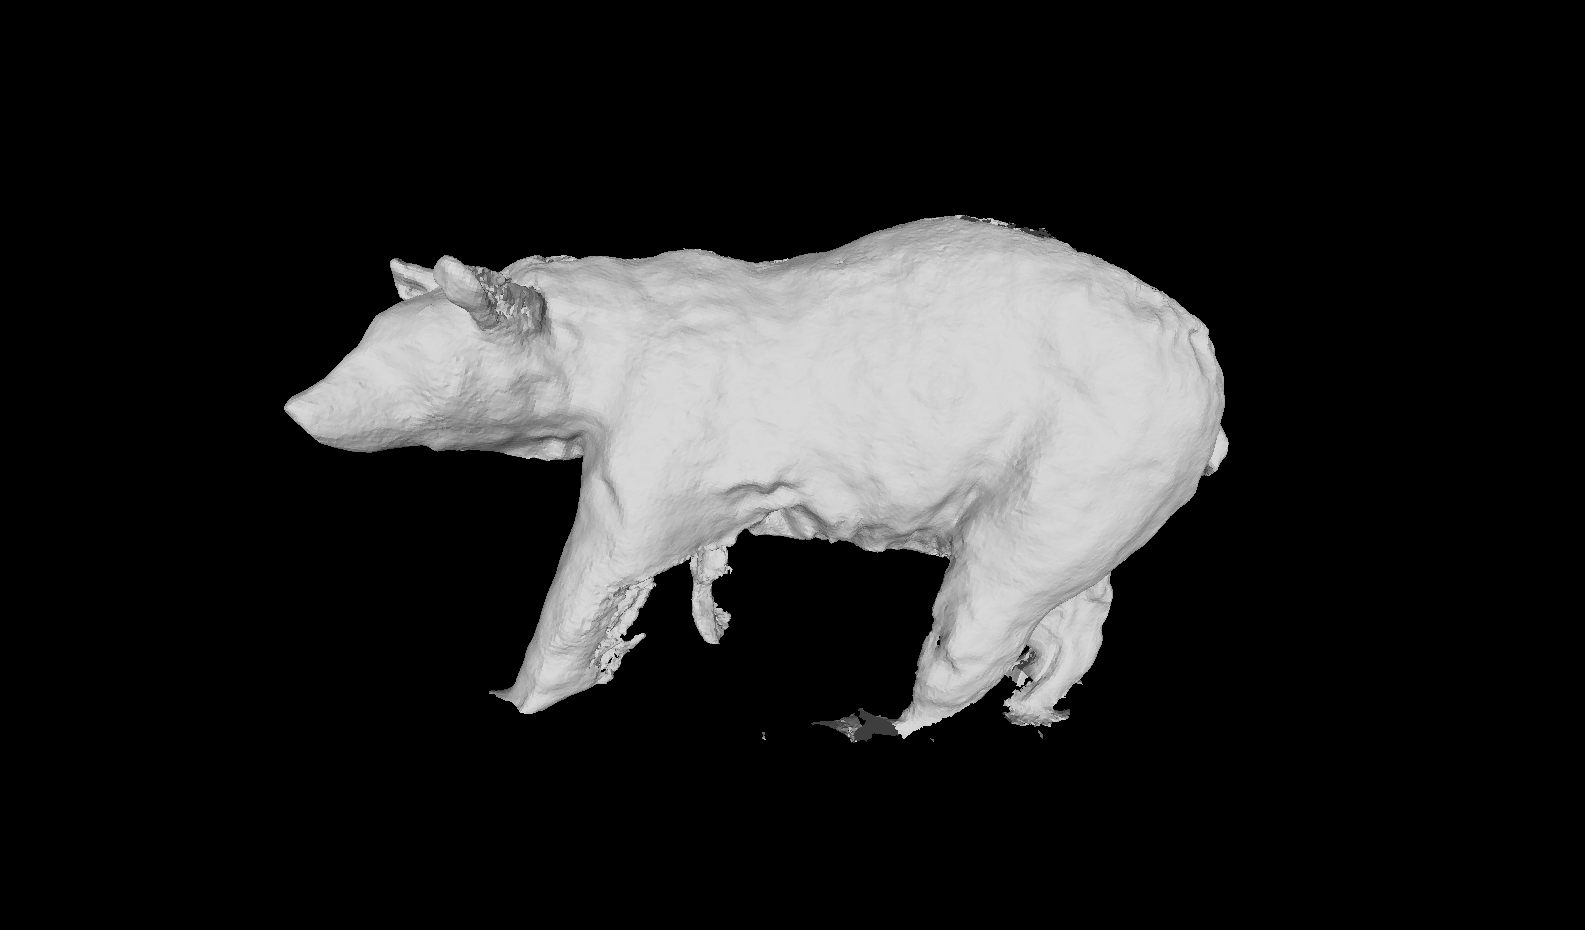
\includegraphics[width=.2\linewidth]{figures/object_recon/comp/itm/bear00.png}&
		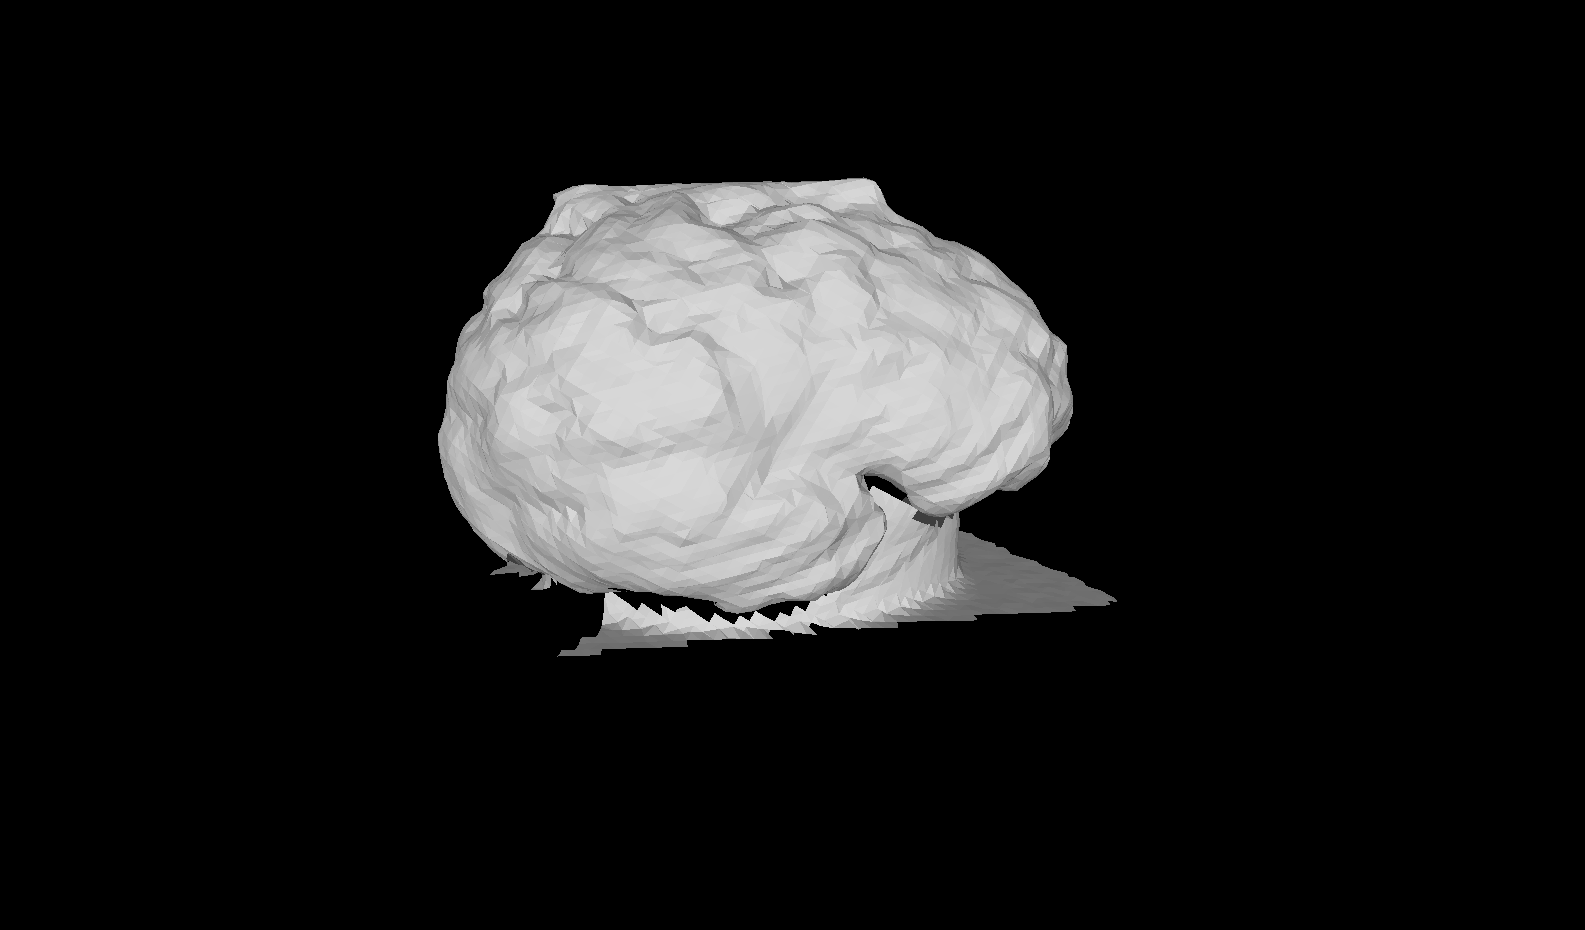
\includegraphics[width=.2\linewidth]{figures/object_recon/comp/itm/brain00.png}&
		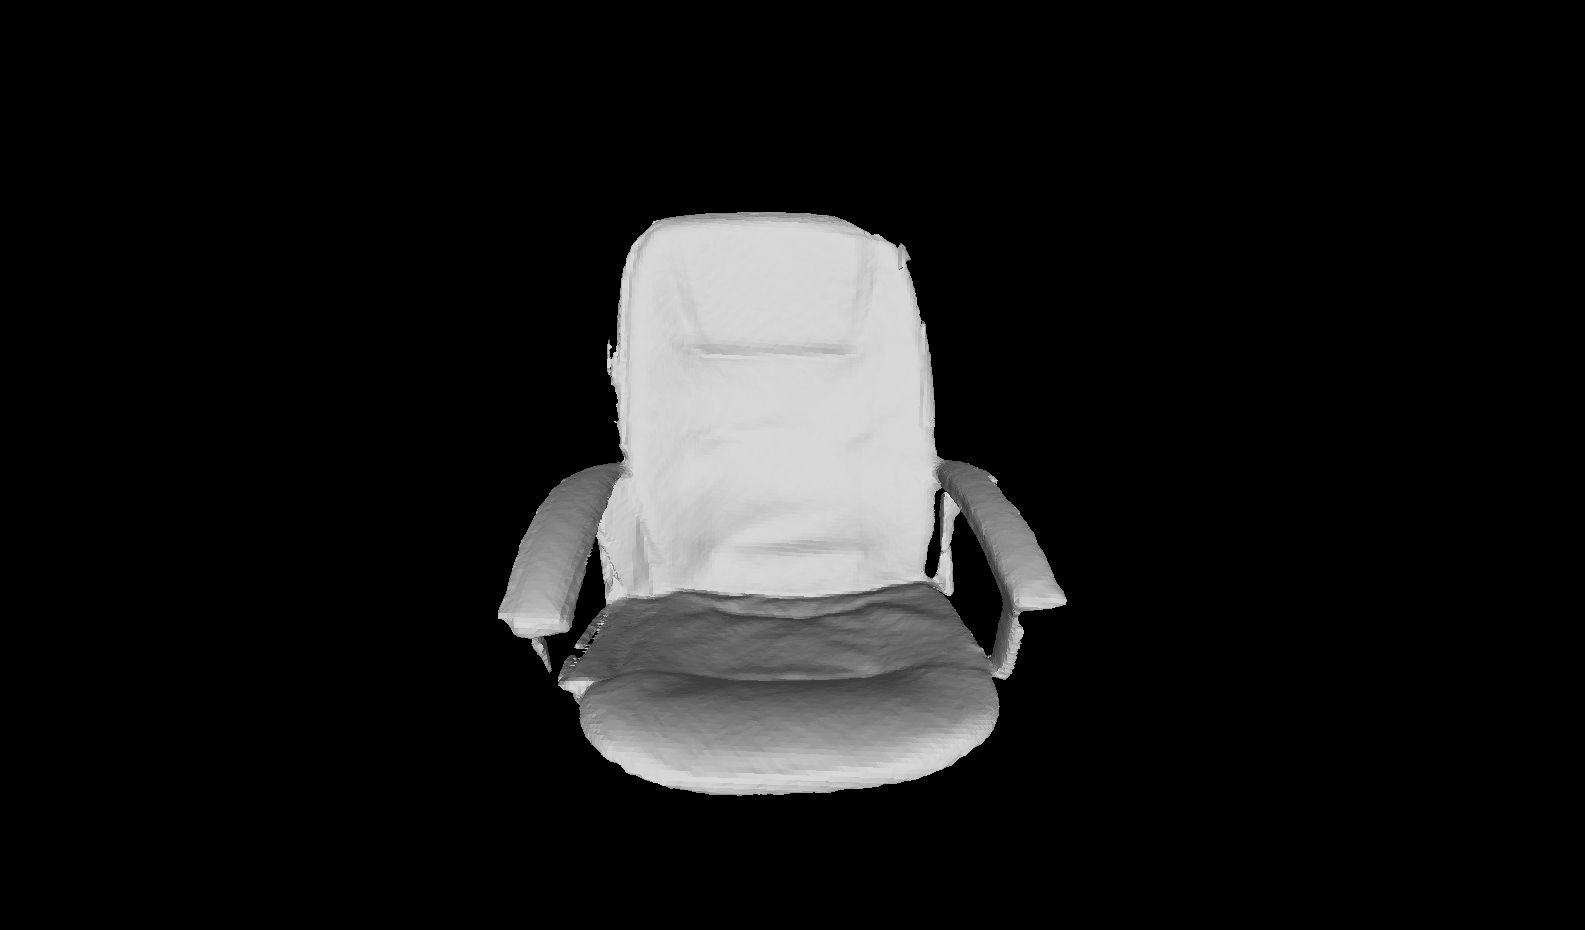
\includegraphics[width=.2\linewidth]{figures/object_recon/comp/itm/chair00.png}&
    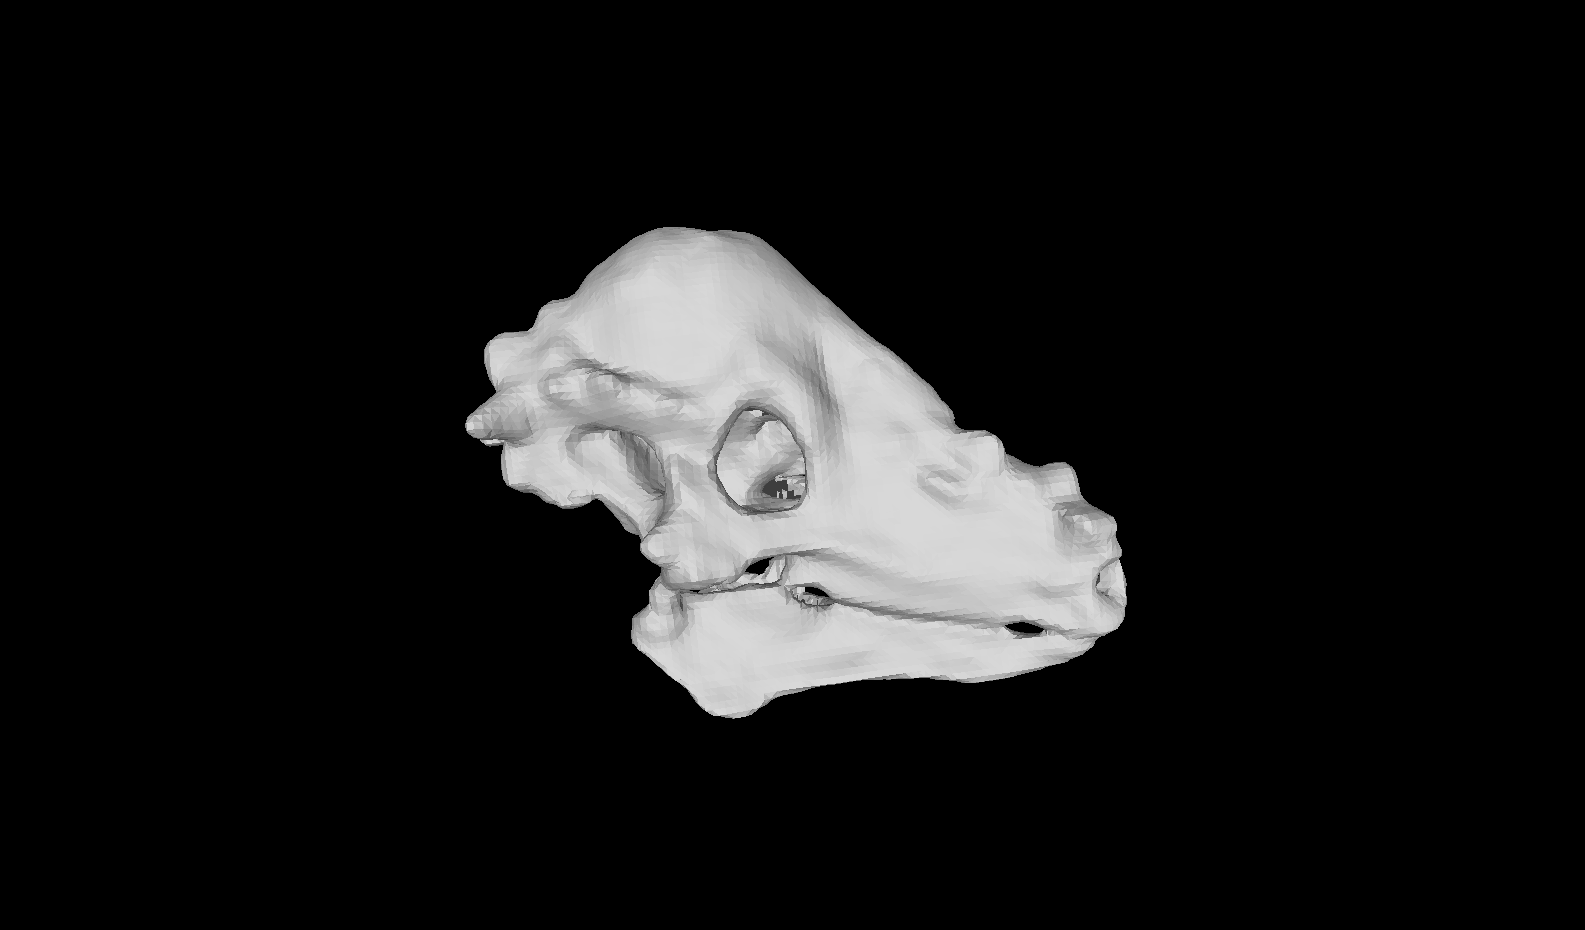
\includegraphics[width=.2\linewidth]{figures/object_recon/comp/itm/dino00.png} \\
    (a) & (b) & (c) & (d) \\
		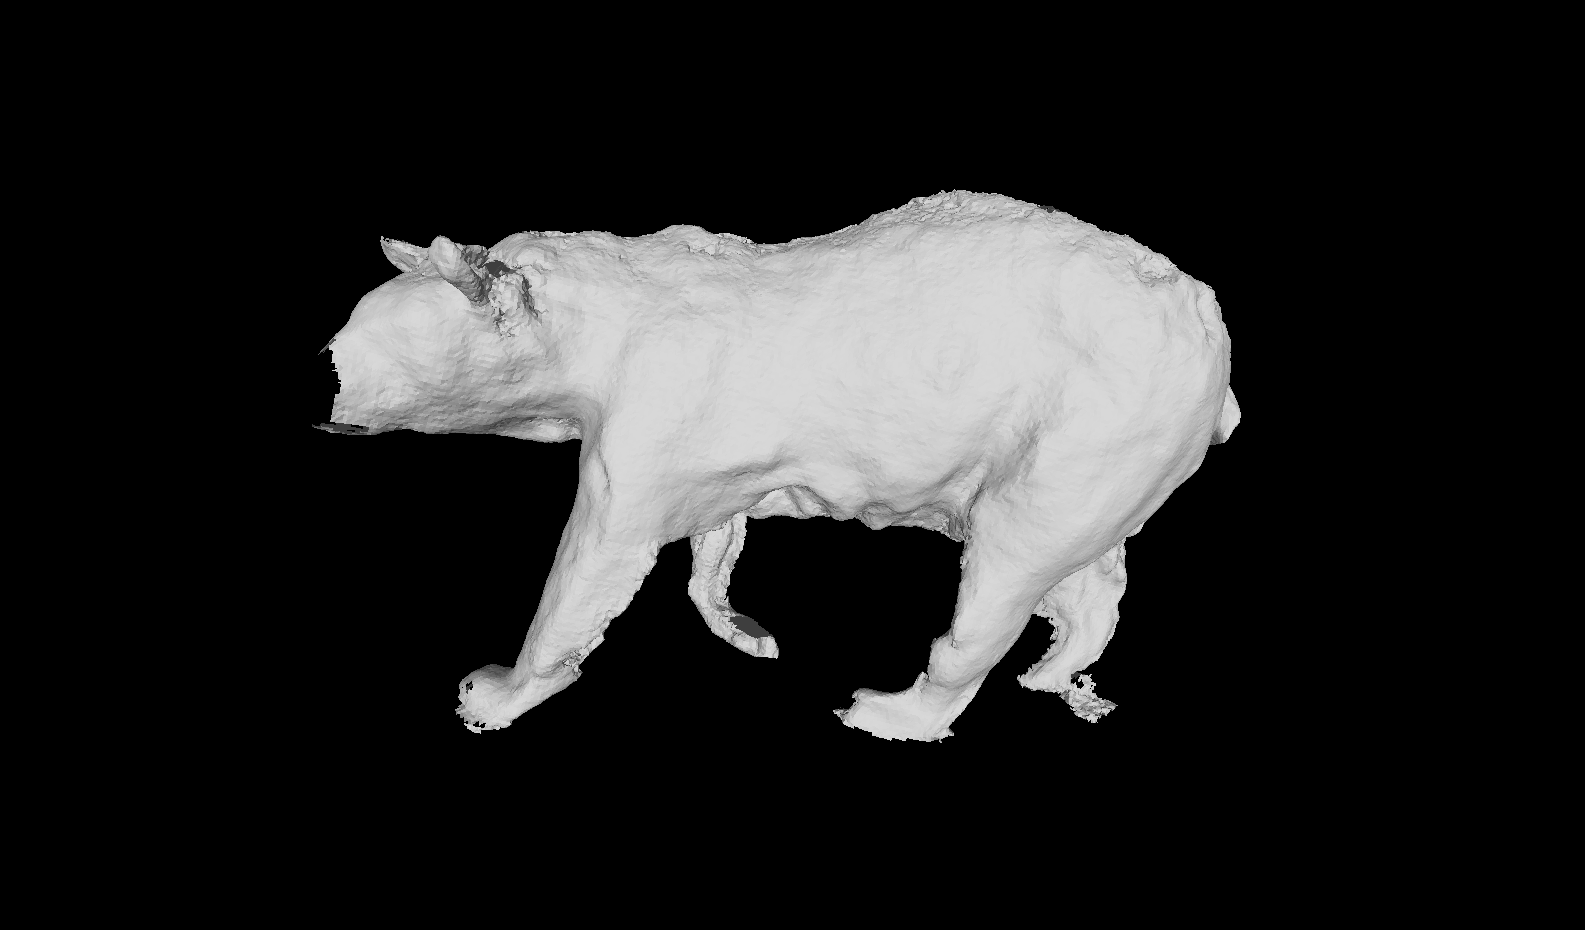
\includegraphics[width=.2\linewidth]{figures/object_recon/comp/prob/bear00.png}&
		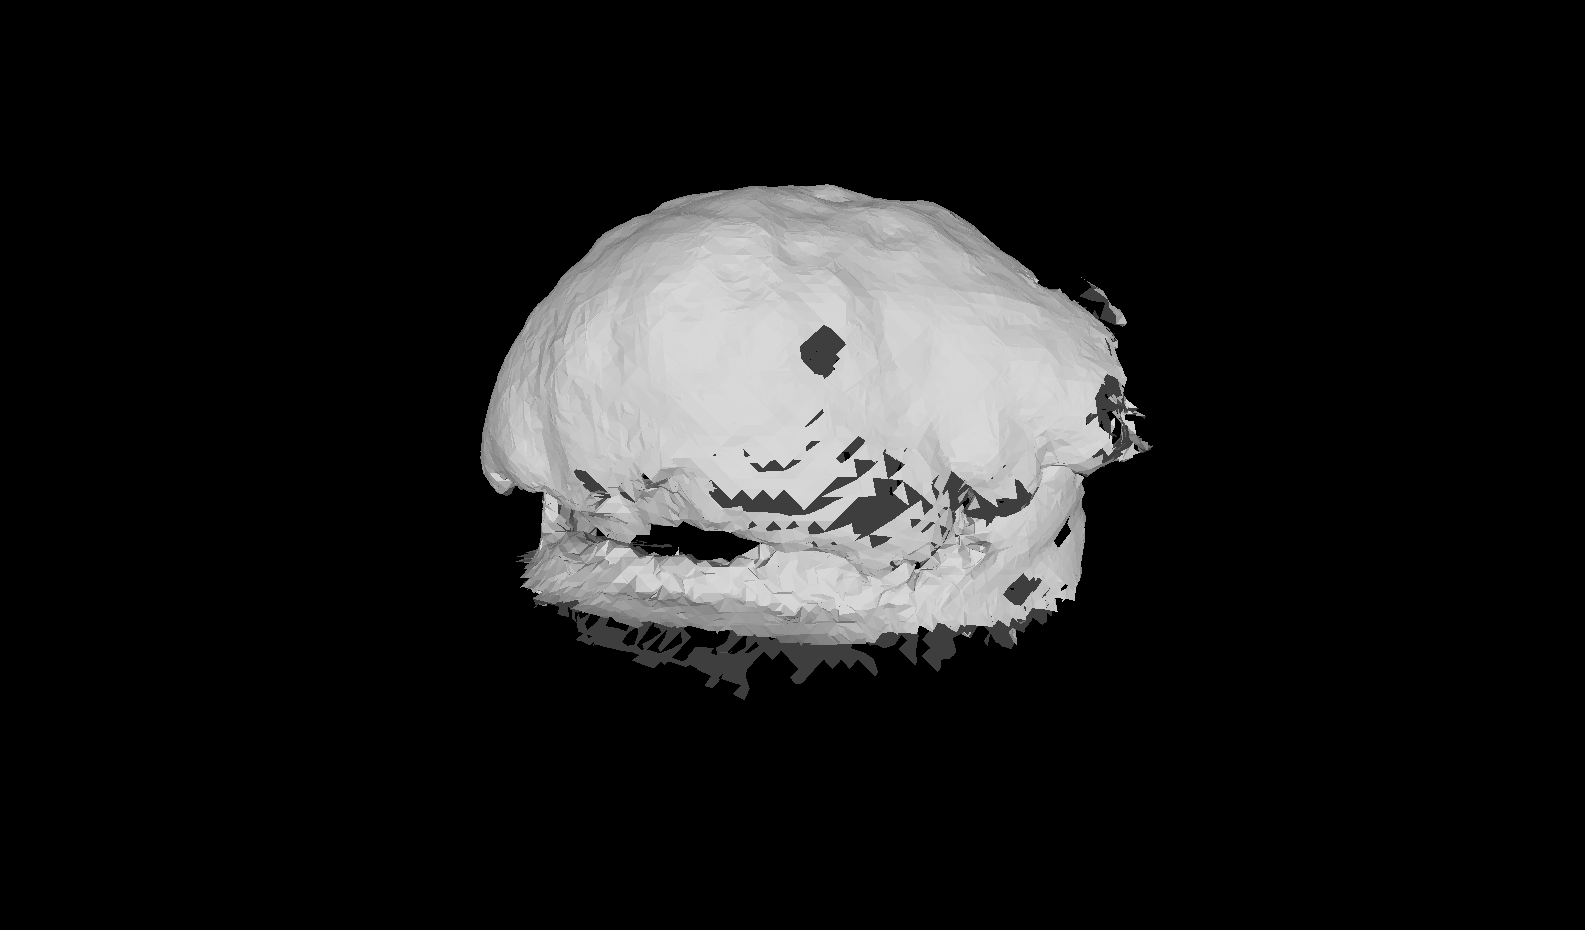
\includegraphics[width=.2\linewidth]{figures/object_recon/comp/prob/brain00.png}&
		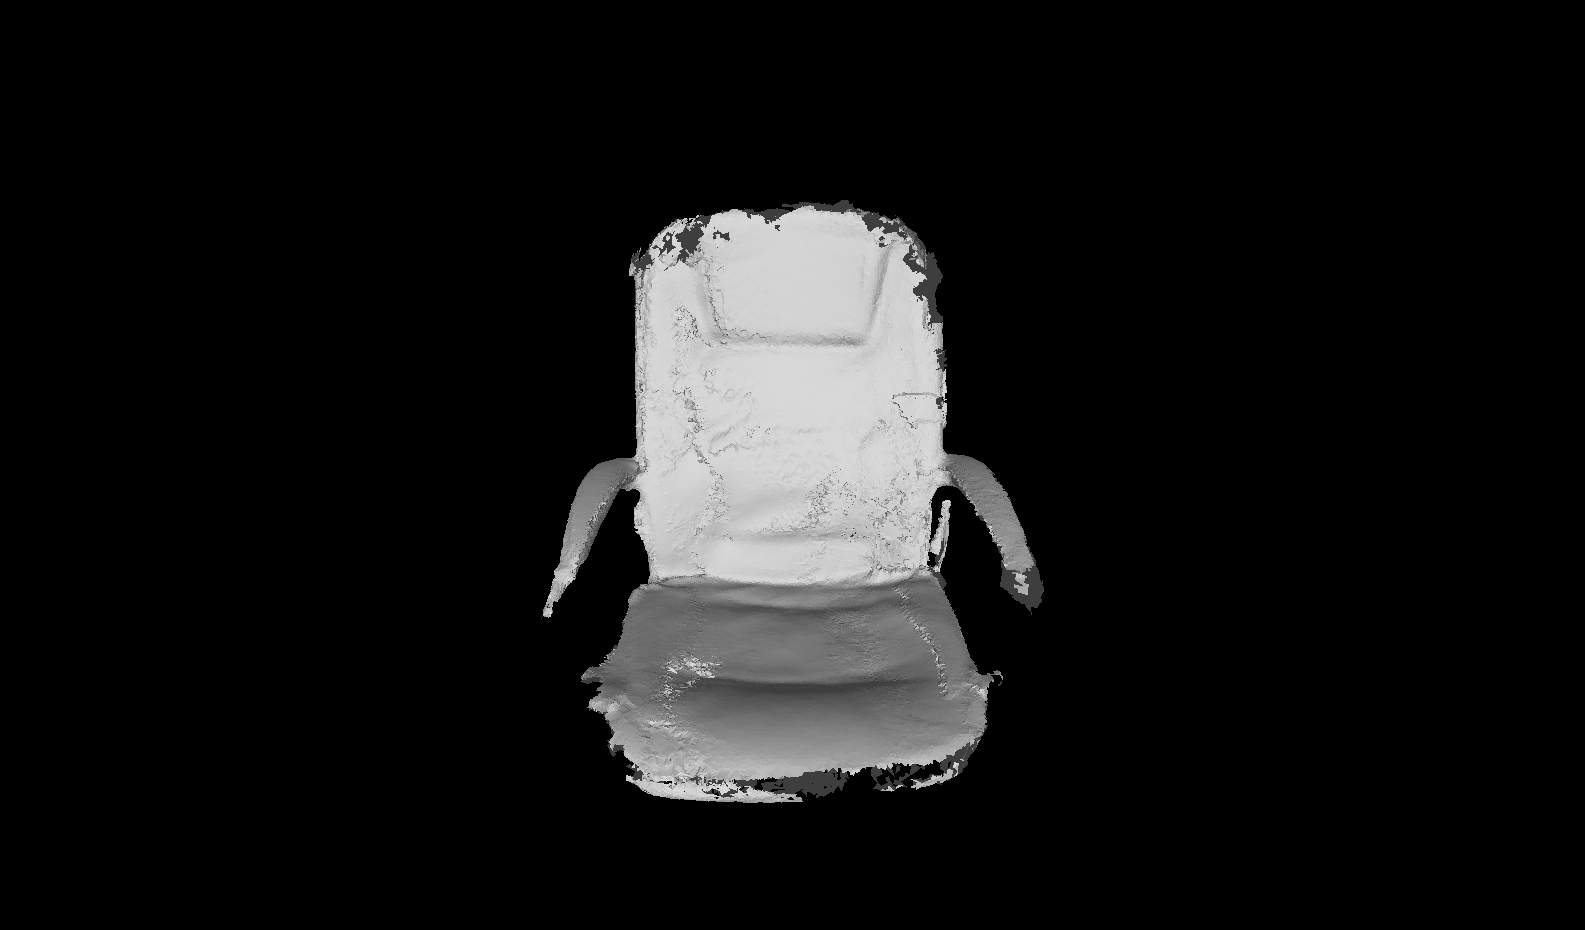
\includegraphics[width=.2\linewidth]{figures/object_recon/comp/prob/chair00.png}&
    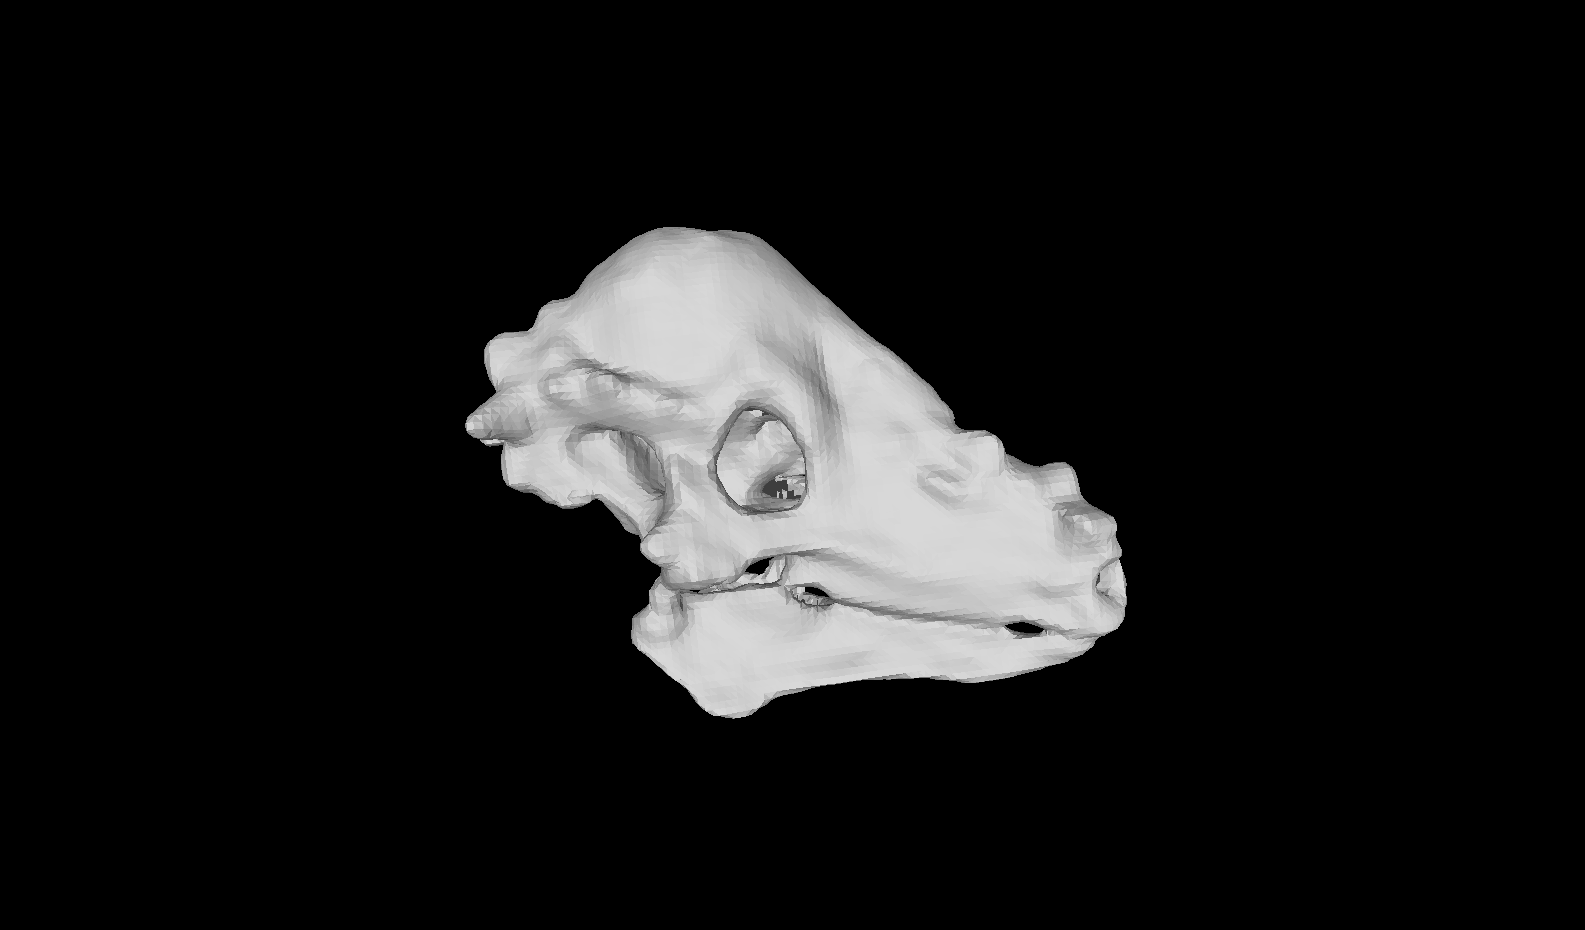
\includegraphics[width=.2\linewidth]{figures/object_recon/comp/itm/dino00.png} \\
    (e) & (f) & (g) & (h) \\
  \end{tabular}
  \caption[Probabilistic Object Reconstruction Qualitative Results III]
  {(a, b, c, d) Base reconstructions extracted from the output of the 
  standard KinectFusion pipeline. (e, f, g, h) Reconstructions yielded by 
  the proposed approach.}
\end{figure}

As can be seen in Figure \ref{fig:probobj_comp_itm} the proposed system is 
capable of providing reconstructions of a wide variety of objects in an 
aesthetically similar manner to a well established baseline. The proposed 
system provides globally consistent, closed reconstructions as is evident from 
the top-down views presented in Figure \ref{fig:probobj_comp_itm}.

\begin{figure}[h]
  \label{fig:probobj_comp_itm}
	\centering
	\begin{tabular}{cccc}
		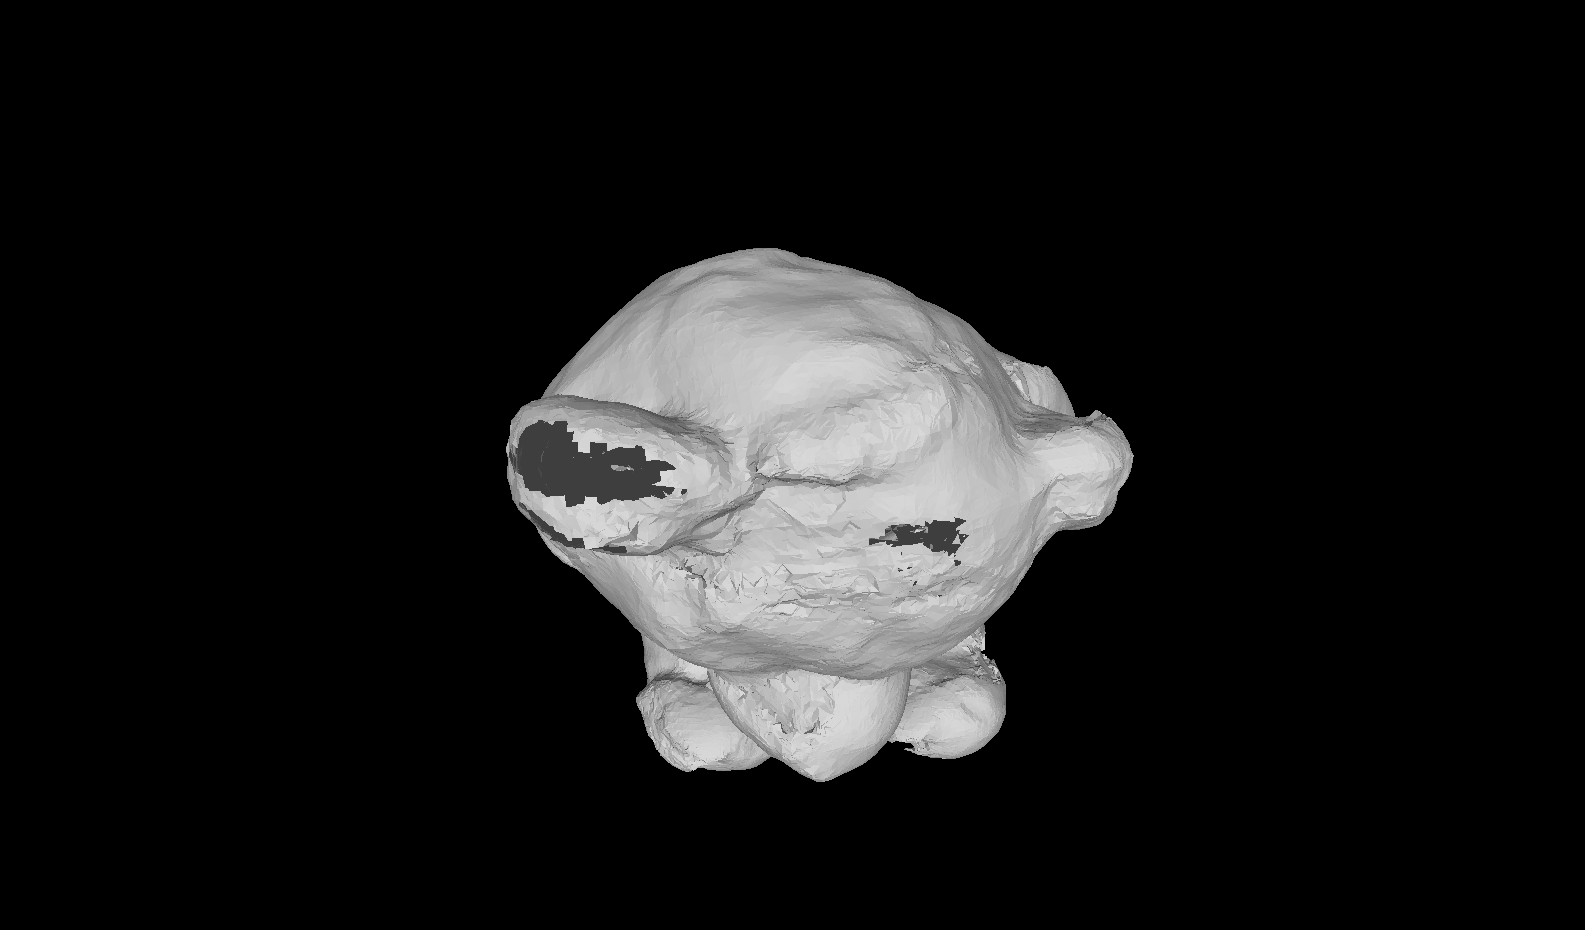
\includegraphics[width=.2\linewidth]{figures/object_recon/top/teddy_top00.png}&
    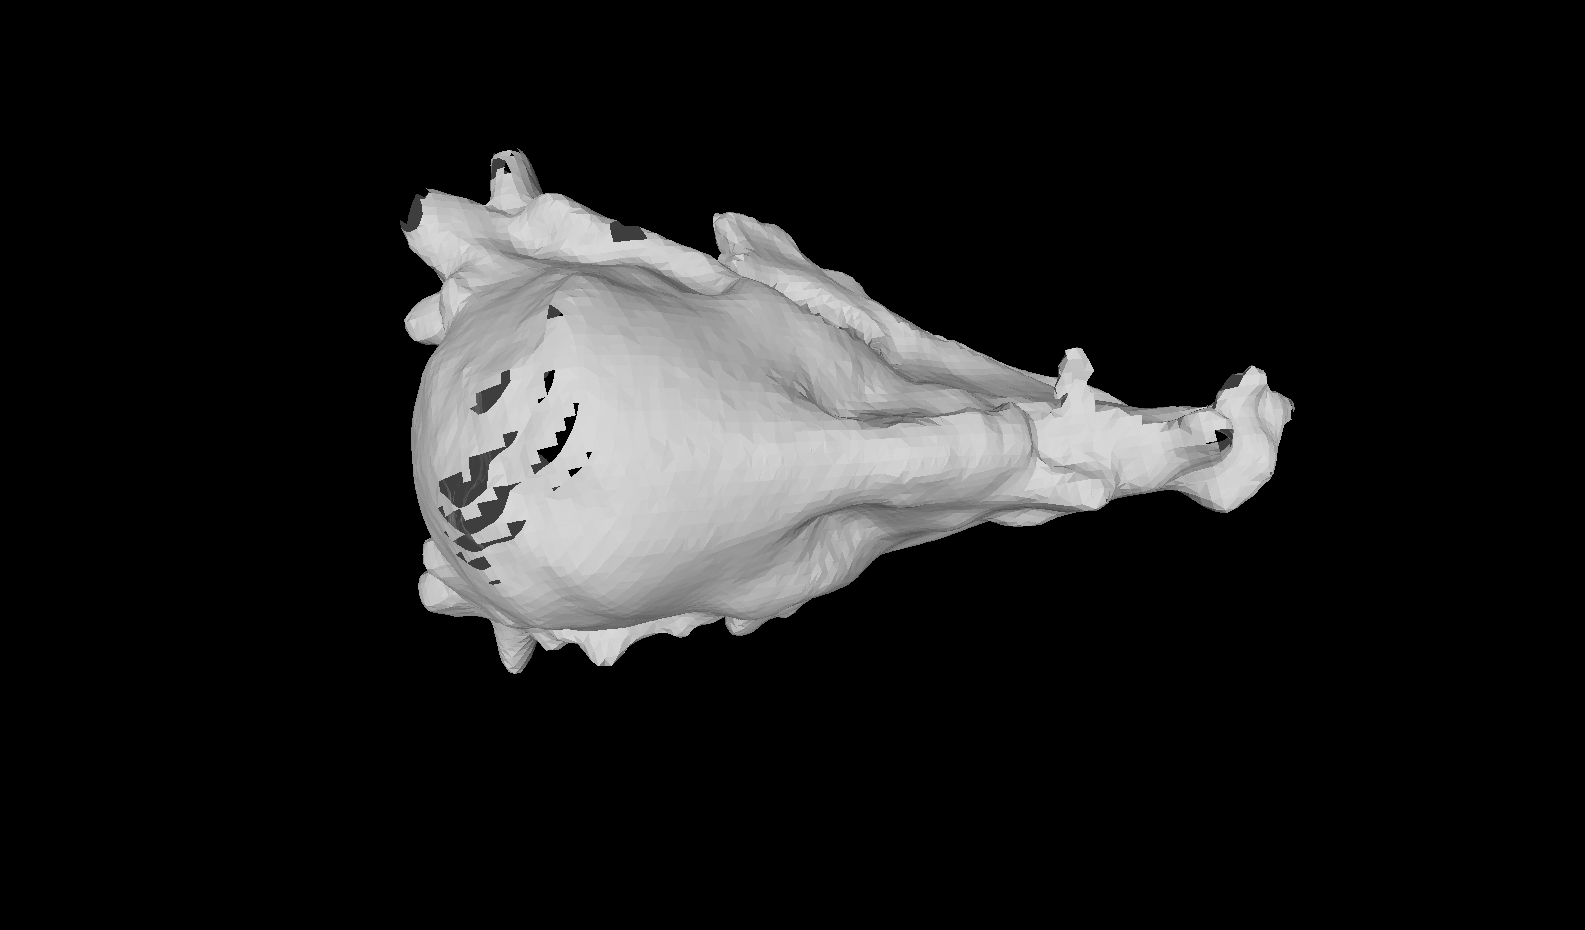
\includegraphics[width=.2\linewidth]{figures/object_recon/top/dino_top00.png} &
		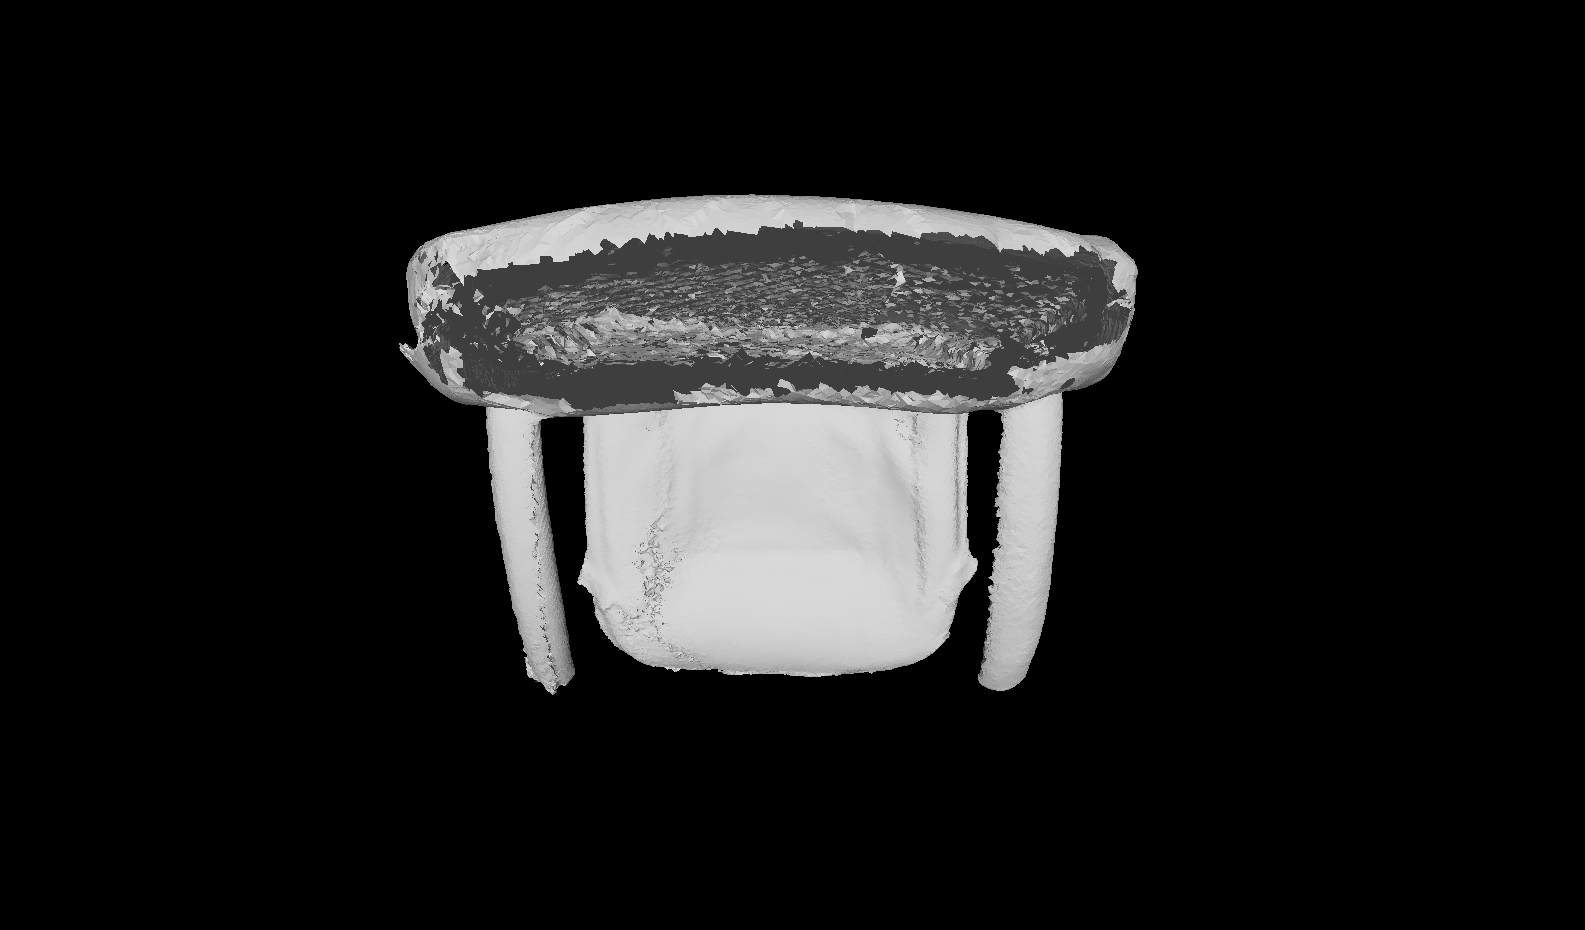
\includegraphics[width=.2\linewidth]{figures/object_recon/top/chair_top00.png}&
    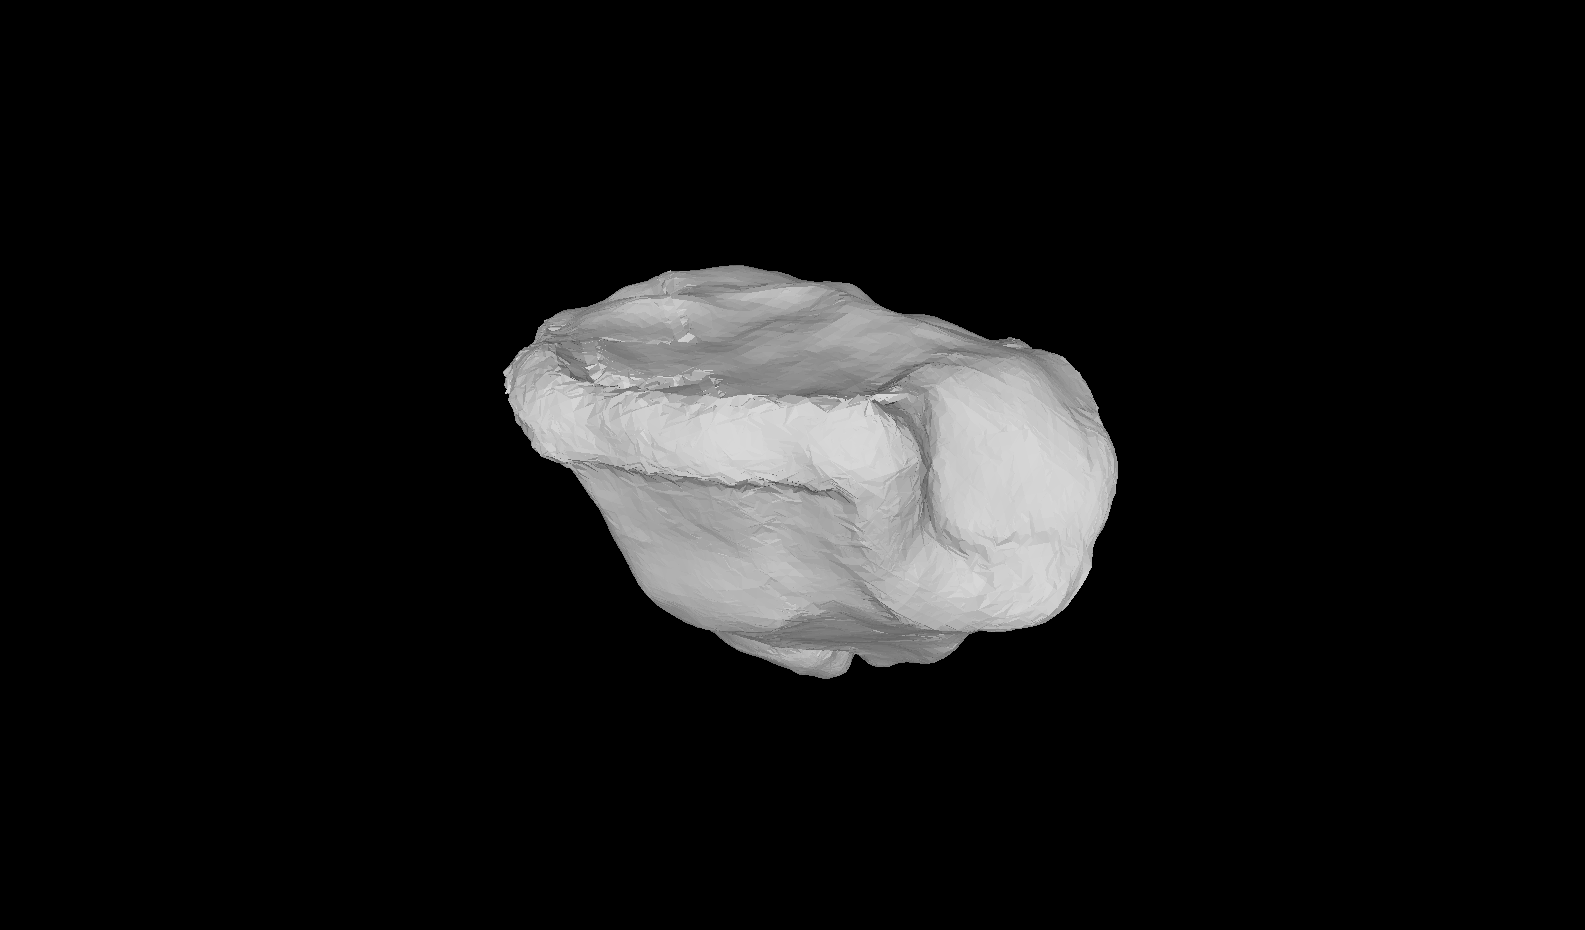
\includegraphics[width=.2\linewidth]{figures/object_recon/top/rock_top00.png} \\
    (a) & (b) & (c) & (d) \\
	\end{tabular}
  \caption[Probabilistic Object Reconstruction Qualitative Results IV]
  {
    Closed reconstructions of the (a) Teddy, (b) Dinosaur Head, 
    (c) Chair and (d) Rock sequences.
	}
\end{figure}

The efficacy of the approach described in this work is further demonstrated when comparing
the pipeline as outlined in Figure \ref{fig:probobj_pipeline_diagram} to a version that 
utilises only a single representation of the object of interest. Figure 
\ref{fig:probobj_gappy_teddy} demonstrates the difference in reconstruction output when 
not utilising the multiple subvolume representation and it's accompanying enforcement 
of consistency constraints. 

\begin{figure}[h]
  \label{fig:probobj_gappy_teddy}
	\centering
	\begin{tabular}{cc}
		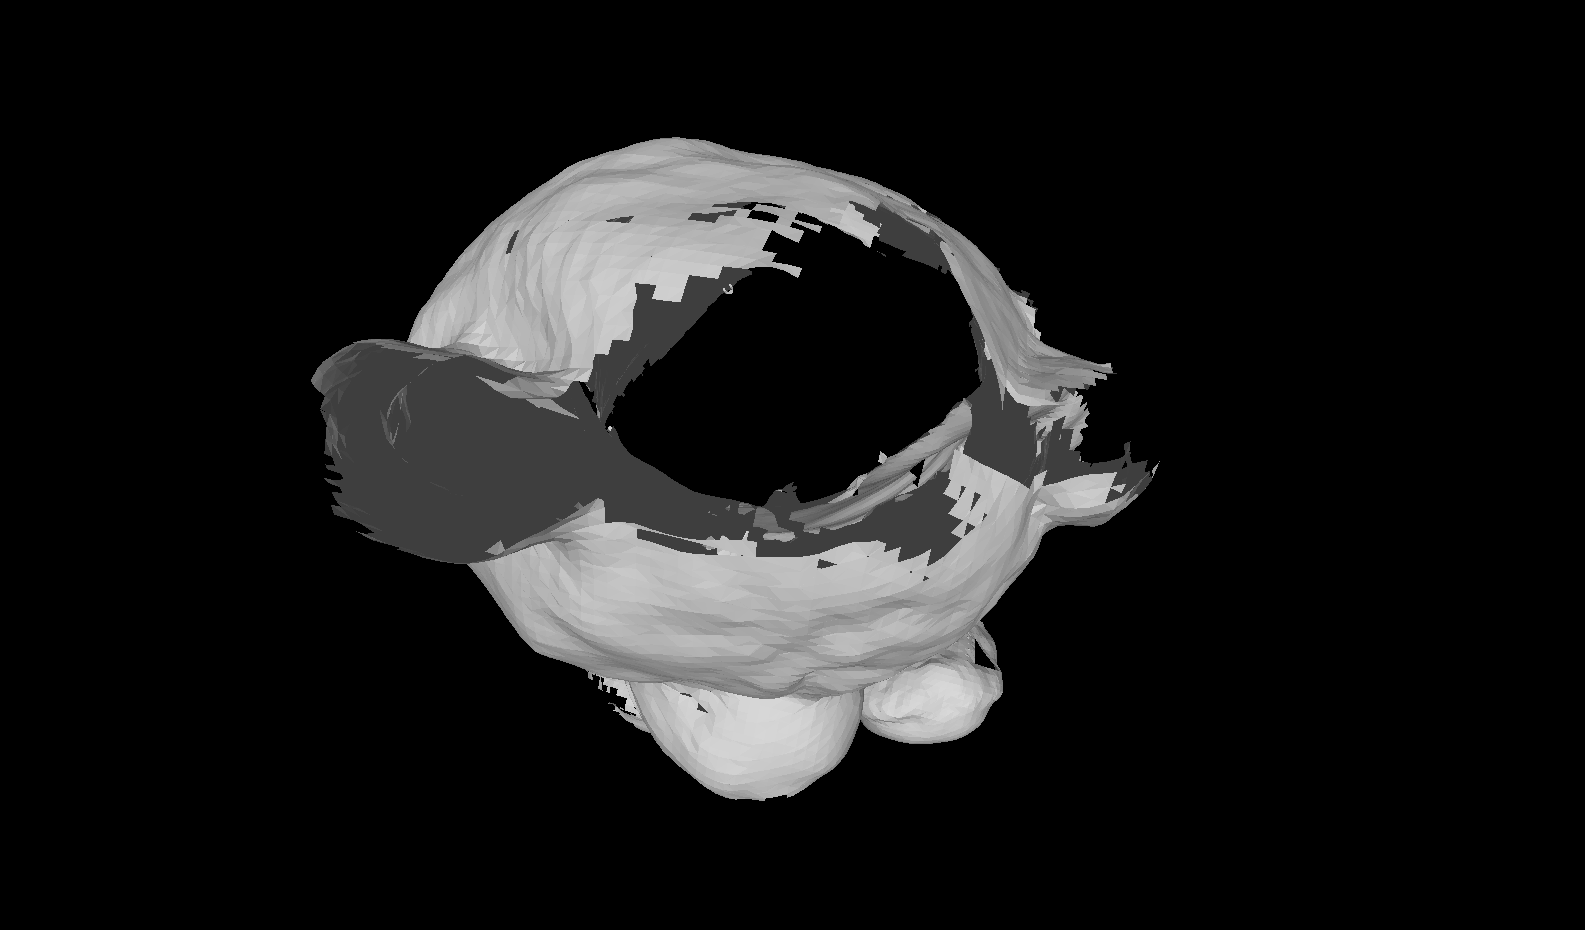
\includegraphics[width=.2\linewidth]{figures/object_recon/gappy/one_scene00.png}&
    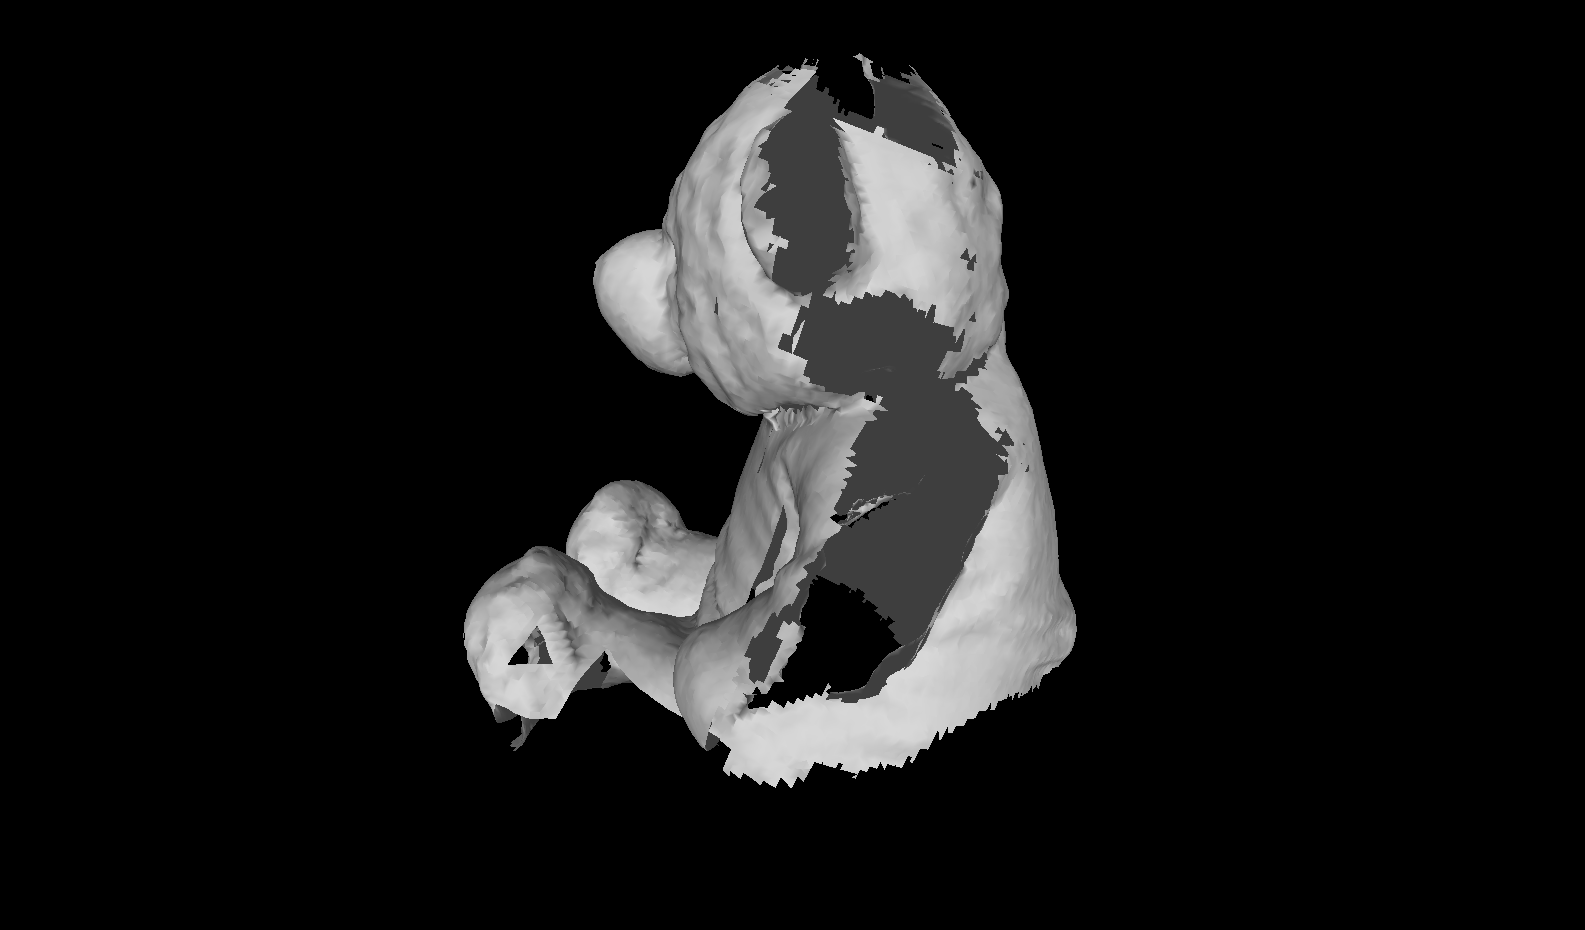
\includegraphics[width=.2\linewidth]{figures/object_recon/gappy/one_scene01.png}\\
    (a) & (b) \\
		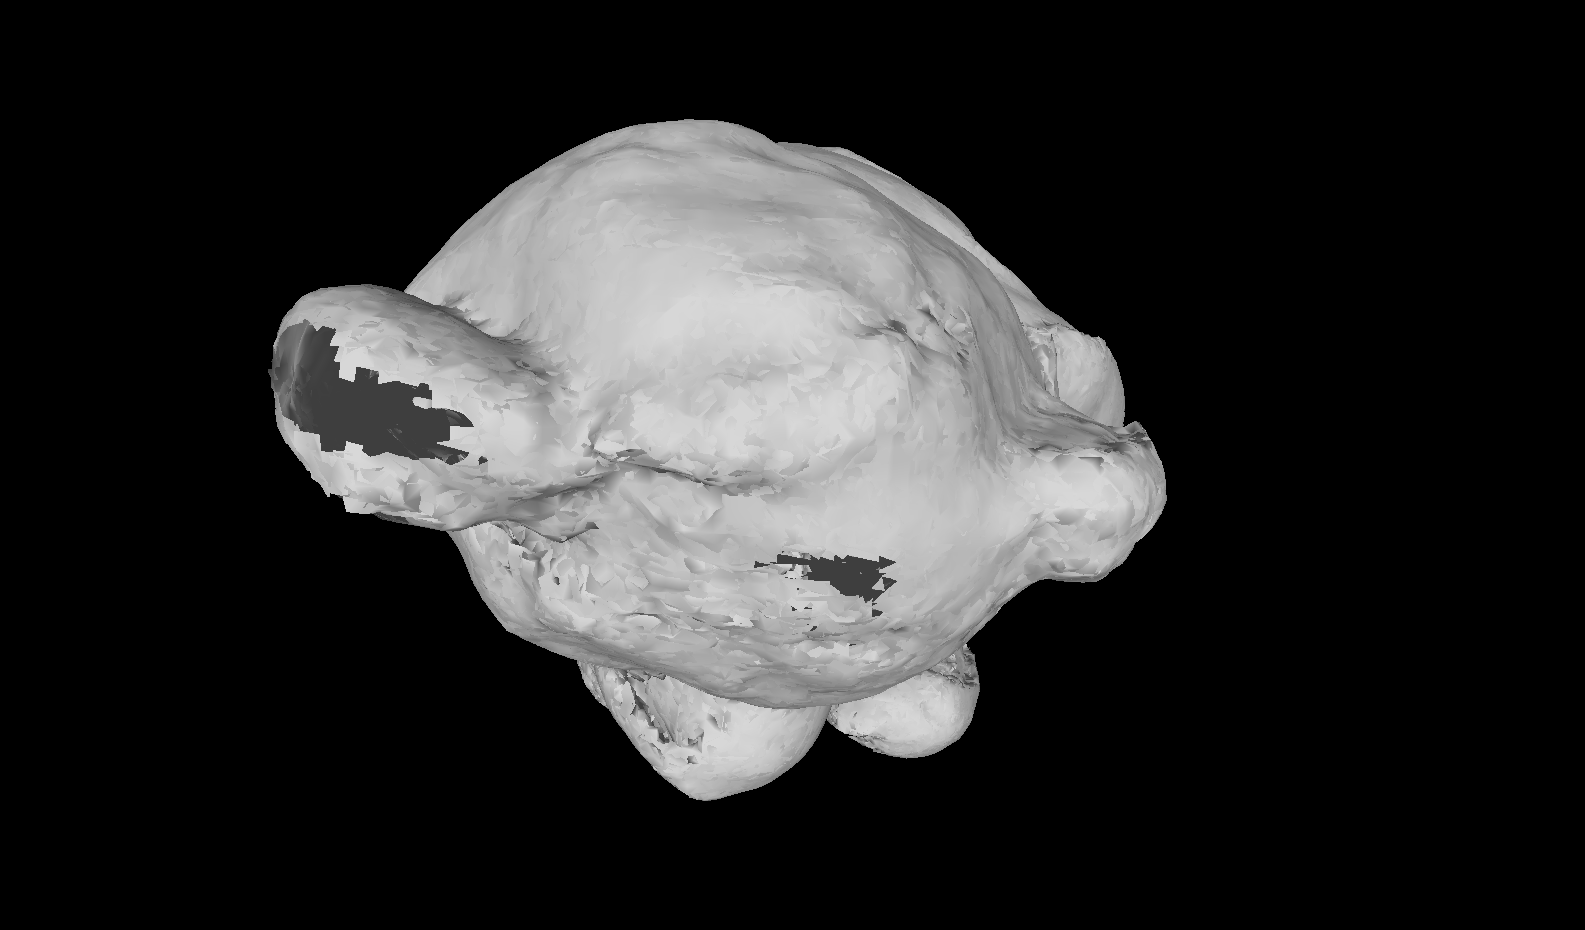
\includegraphics[width=.2\linewidth]{figures/object_recon/gappy/multi_scene00.png}&
    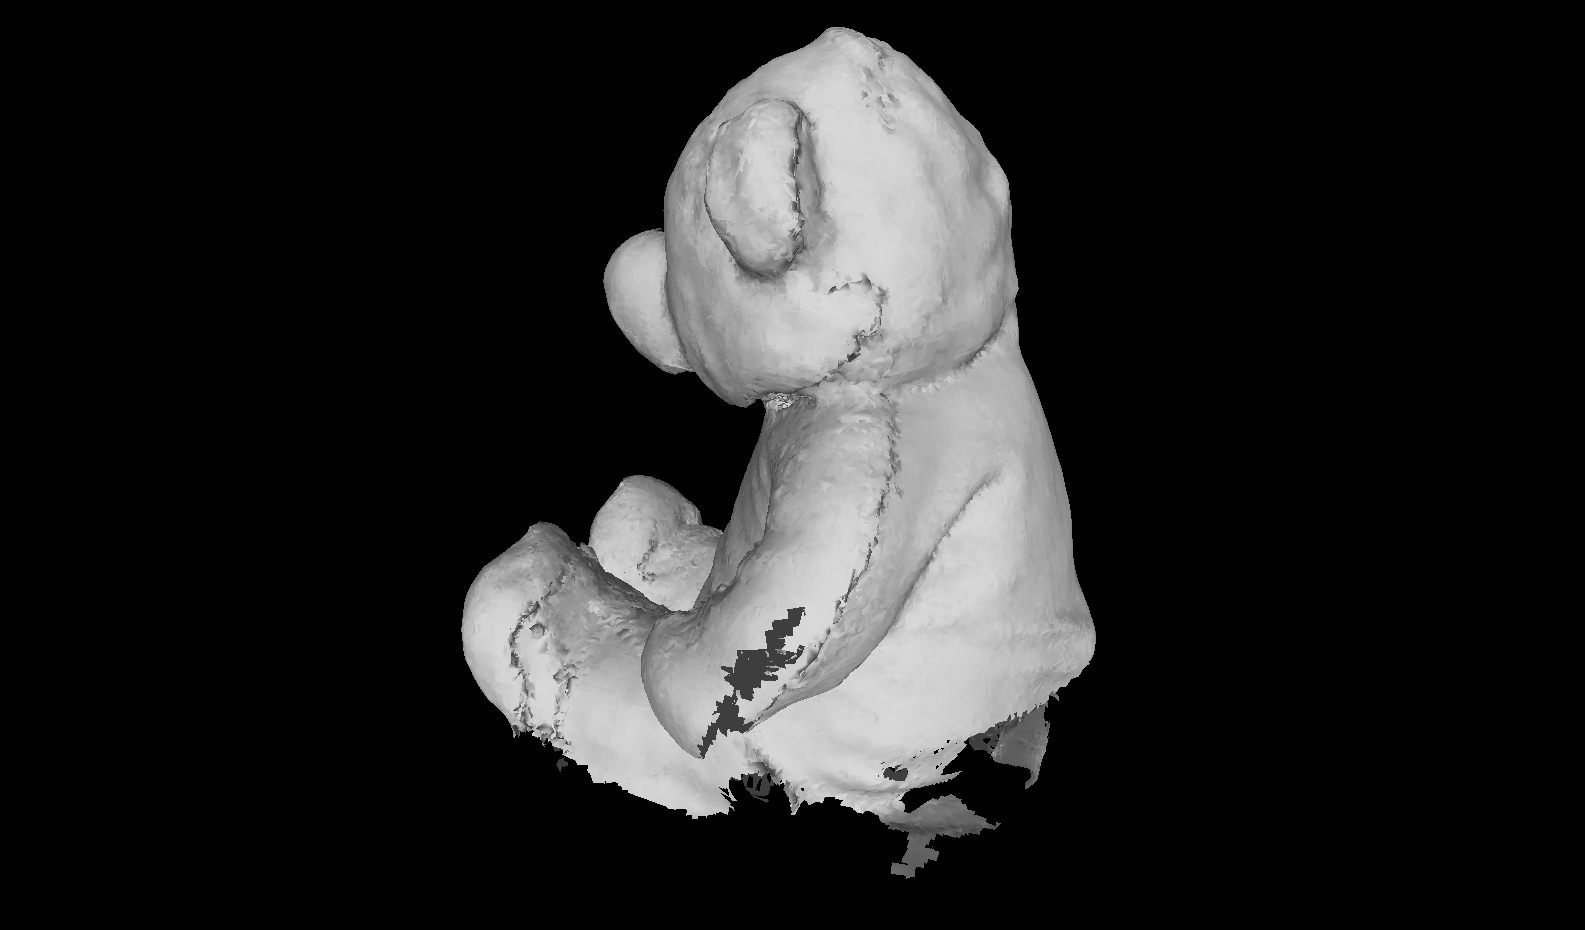
\includegraphics[width=.2\linewidth]{figures/object_recon/gappy/multi_scene01.png}\\
    (c) & (d)\\
	\end{tabular}
  \caption[Probabilistic Object Reconstruction Qualitative Results V]
  {
    Teddy reconstruction with InfiniTAM (a, b) versus the system proposed in this 
    work (c, d).
	}
\end{figure}

The gaps in the isosurface depicted in Figure \ref{fig:probobj_gappy_teddy} (a, b) 
demonstrate the impact that drift in the pose estimation stage can have on the resultant 
reconstruction; drift can incur irregularities in the extraction and rendering of the objects 
isosurface. Note that the reconstructions given in Figure \ref{fig:probobj_gappy_teddy} 
(c, d) do not suffer such irregularities when utilising the object reconstruction pipeline 
presented in this chapter.

\section{Quantitative Results}
\label{sec:probobj_quantitative}
In this section the performance of the proposed system is evaluated quantitatively with respect 
to both pose estimation accuracy and reconstruction accuracy. 

For pose evaluation, the \textit{3D Object Reconstruction} subset of the 
\textit{RGB-D SLAM Dataset and Benchmark} \cite{Sturm2012}. The objects of interest in 
the dataset vary largely in both geometry and appearance. As with the quantitative 
evaluation presented in Section \ref{sec:moseg_quantitative}, the 
\textit{Absolute Trajectory Error} is the primary metric of interest.

\begin{table}[h]
  \label{tbl:probobj_ate}
  \centering
  \begin{tabular}{l@{\hskip 1cm} c c}
    \emph{Sequence Name} & \emph{Proposed Approach ATE (m)} & \emph{InfiniTAM (m)}\\
    \midrule
    \textsf{freiburg3\_cabinet} & 0.077903 & 0.520693\\
    \textsf{freiburg3\_teddy}   & 0.030596 & 0.048560 \\
    \textsf{freiburg1\_plant}   & DNR & DNR \\
    \textsf{freiburg2\_coke}   & DNR & DNR \\
    \textsf{freiburg2\_dishes}   & DNR & DNR \\
    \textsf{freiburg2\_flowerbouquet}   & DNR & DNR \\
    \textsf{freiburg2\_flowerbouquet\_brownbackground}   & DNR & DNR \\
    \textsf{freiburg2\_metallic\_sphere}   & DNR & DNR \\
    \textsf{freiburg2\_metallic\_sphere2}   & DNR & DNR \\
    \textsf{freiburg3\_large\_cabinet}   & DNR & DNR
  \end{tabular}
  \caption[Probabilistic Object Reconstruction ATE]
  {ATE results achieved by the proposed approach versus InfiniTAM with object segmentation.}
\end{table}

It can be seen from Table \ref{tbl:probobj_ate} that on the \textit{freiburg3\_cabinet} 
and \textit{\textsf{freiburg3\_teddy}} sequences the approach proposed in this work 
yields a marked improvement in Absolute Trajectory Error over that of the standard KinectFusion 
pipeline with object segmentation. The remaining sequences that have the ATE marked as DNR did 
not yield an interpretable reconstruction; sequences with ATE metrics marked DNR did not 
reconstruct. In the case of the \textit{freiburg2\_metallic\_sphere(2)} sequences...

The trajectories of the two approaches evaluated on the \textit{freiburg3\_cabinet} 
and \textit{\textsf{freiburg3\_teddy}} sequences are plotted versus the ground truth trajectories 
in Figure \ref{fig:probobj_traj}

\begin{figure}[h]
  \label{fig:probobj_traj}
  \centering
  \begin{tabular}{cc}
  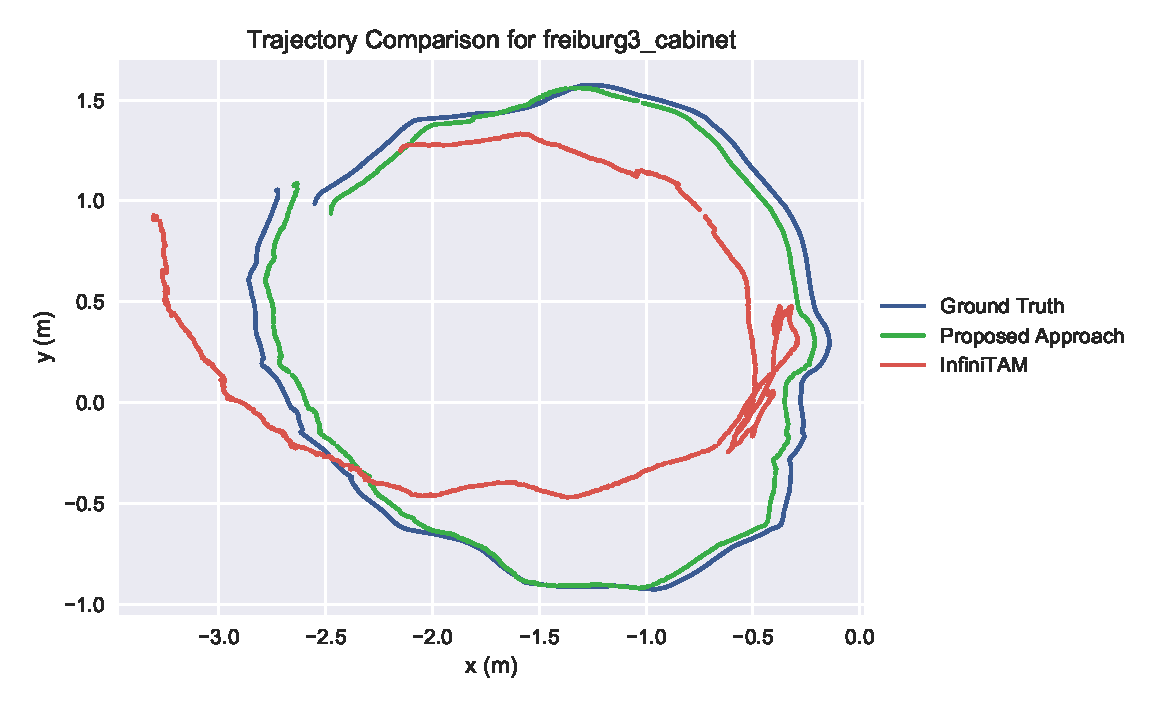
\includegraphics[width=.5\linewidth]{figures/object_recon/plots/traj/cab_traj.eps} & 
  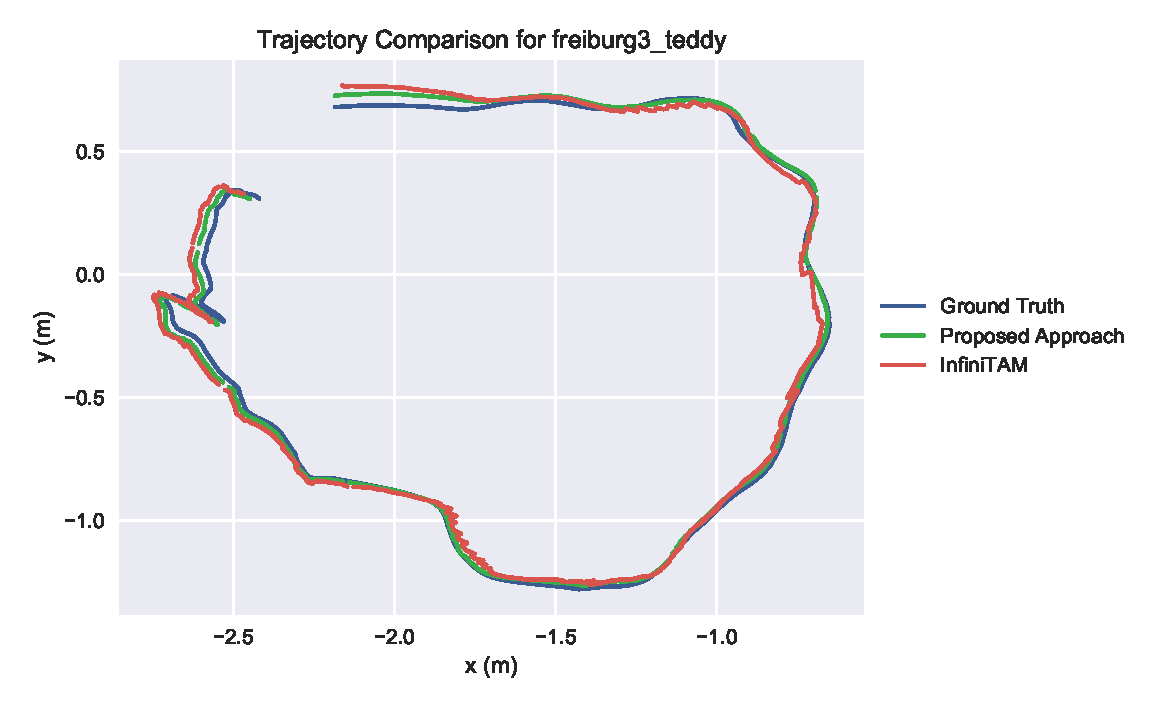
\includegraphics[width=.5\linewidth]{figures/object_recon/plots/traj/ted_traj.eps} \\
  (a) & (b)
  \end{tabular}
  \caption[Probabilistic Object Reconstruction Trajectory Plots]
  {Trajectory plots for the \textit{freiburg3\_cabinet} (a) 
  and \textit{\textsf{freiburg3\_teddy}} (b) sequences.}
\end{figure}

The proposed system is additionally evaluated quantitatively with respect to reconstruction 
quality. Reference models are obtained by reconstructing both the object of interest and it's 
surrounding scene (for maximal Pose Estimation accuracy), followed by a manual segmentation of 
the object of interest in 3-space. To quantify the reconstruction quality the Hausdorff 
Distance \cite{Hausdorff} for subsets of metric spaces is used, where in this case the metric 
space is Euclidean. The Hausdorff Distance is defined as follows in Equation \ref{eqn:probobj_hauss}
\begin{equation}
  \label{eqn:probobj_hauss}
  d_{H}(X, Y) = \max \Bigg[
  \sup_{x \in X} \inf_{y \in Y} d(x, y), \sup_{y \in Y} \inf_{x \in X} d(x, y) 
  \Bigg]
\end{equation}
In Equation \ref{eqn:probobj_hauss}, $X$ is the ground truth dense SLAM reconstruction, 
$Y$ is the reconstruction outputted by the proposed system and $d(.)$ is the Euclidean 
distance.

The resultant quantitative comparisons may be found in Table \ref{tbl:probobj_hauss}.
\begin{table}[h]
  \label{tbl:probobj_hauss}
  \centering
  \begin{tabular}{lcccc}
    \emph{Sequence} & \emph{Min Dist} & \emph{Max Dist} & \emph{Mean Dist} & \emph{RMS}\\
    \midrule
    \textsf{Bear} & 0 & 0.102777 & 0.013588 & 0.019796 \\
    \textsf{Brain} & 0 & 0.026465 & 0.008745 & 0.011349 \\
    \textsf{Chair} & 0 & 0.053441 & 0.012349 & 0.016422 \\
    \textsf{Dinosaur Head} & 0 & 0.035252 & 0.007919 & 0.010676
  \end{tabular}
  \caption[Probabilistic Object Reconstruction Hausdorff Distance]
  {Minimum, maximum, mean and RMSE distances between the reconstructions yielded by 
  the proposed system and the baseline.}
\end{table}

As can be seen by the similarity measures presented, the proposed system is capable of 
yielding reconstructions to a high quality despite the markedly more difficult pose estimation 
scenario of utilising the observations of a single object rather than those an entire scene. 
It can be seen that the presented output reconstructions are geometrically close to those 
reconstructed with a dense SLAM system \cite{Prisacariu2014} following the KinectFusion 
\cite{Newcombe2011} pipeline that is modelling and tracking the entire scene and thus has 
much more geometrical data with which to estimate pose.

Figure \ref{fig:probobj_hauss} presents renderings of the \textit{Teddy}, 
\textit{Brain}, \textit{Chair} and \textit{Dinosaur Head} sequences textured 
on the Haussdorf Distance between the output reconstructions of the presented 
system and the base reconstructions extracted from the KinectFusion like pipeline.

\begin{figure}[h]
  \label{fig:probobj_hauss}
  \centering
  \begin{tabular}{@{}c@{}}
    \begin{tabular}{cccc}
      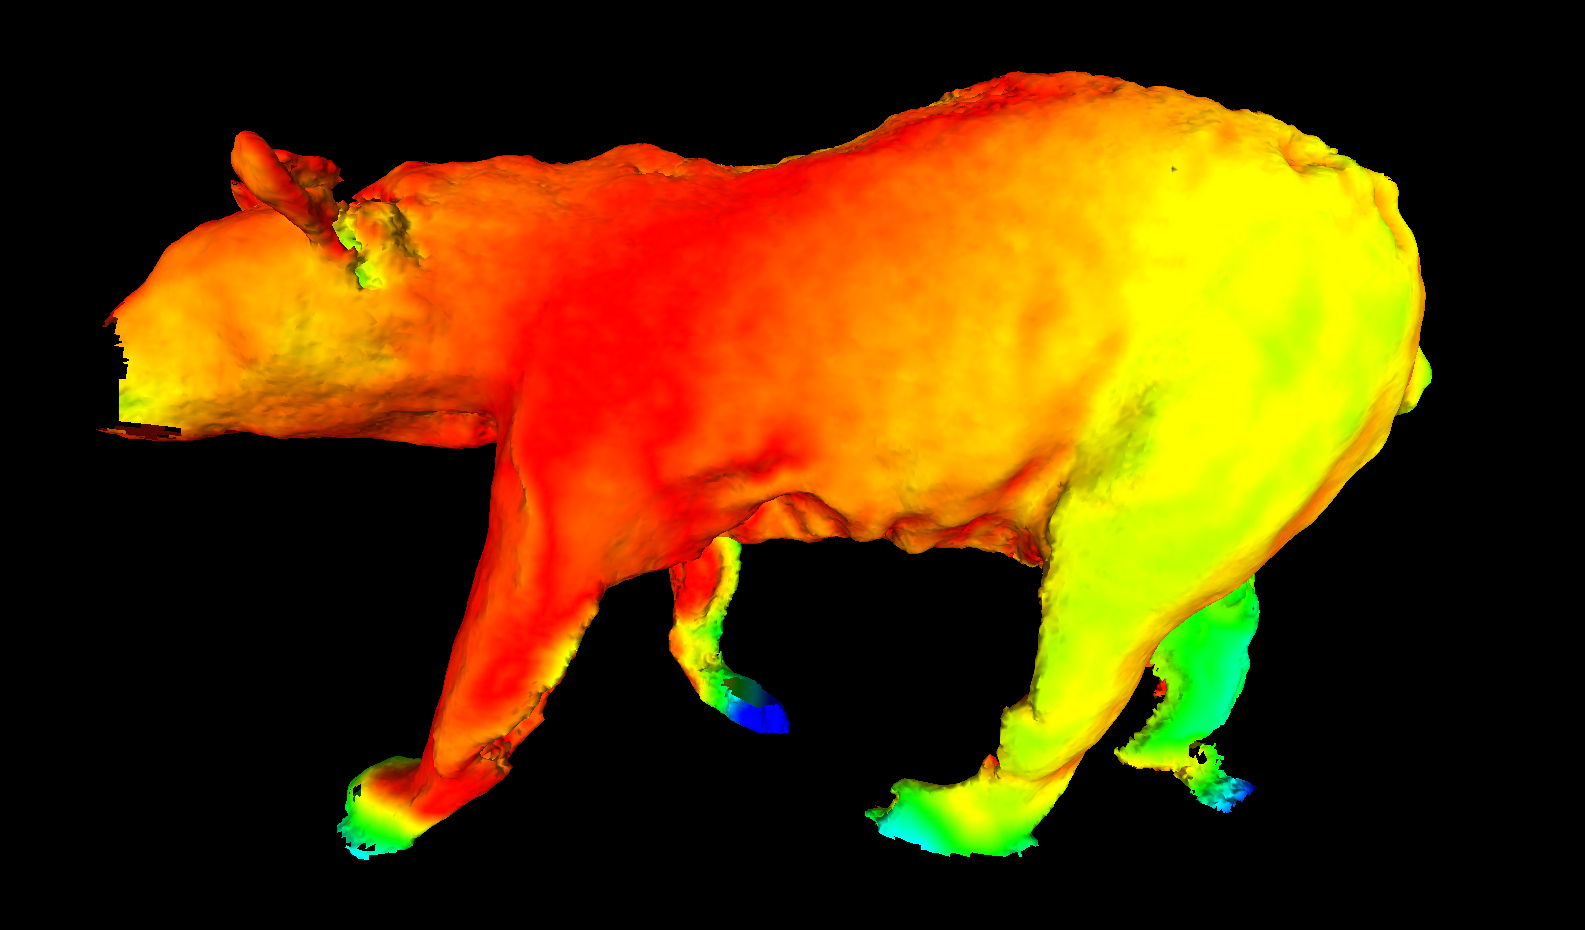
\includegraphics[width=.2\linewidth]{figures/object_recon/hauss/bear.png}&
      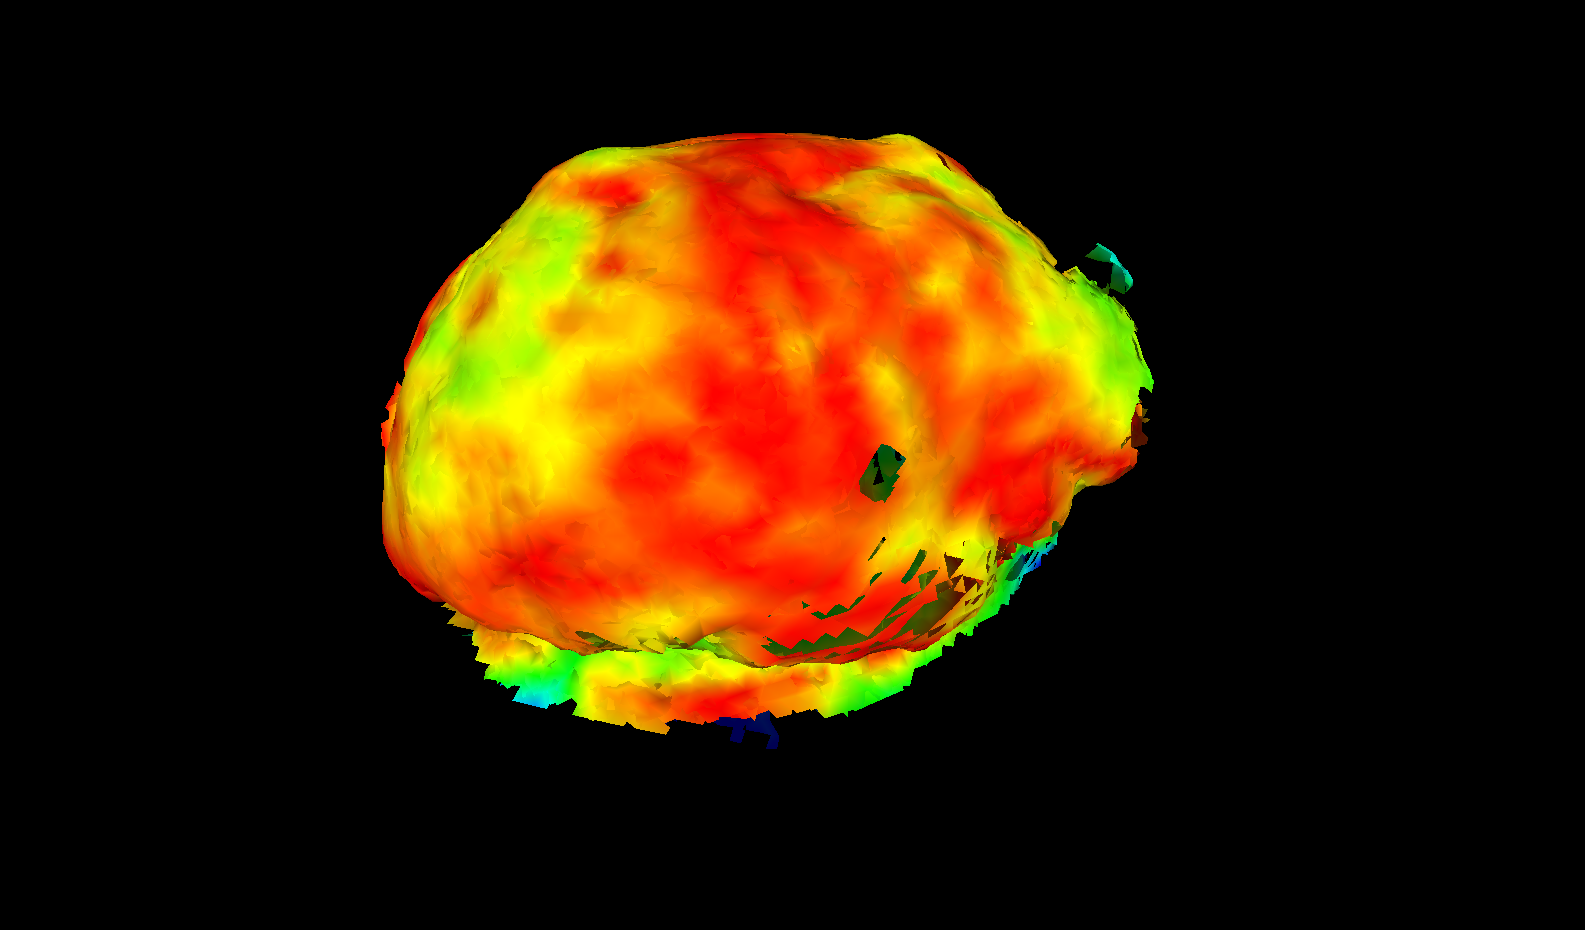
\includegraphics[width=.2\linewidth]{figures/object_recon/hauss/brain.png}&
      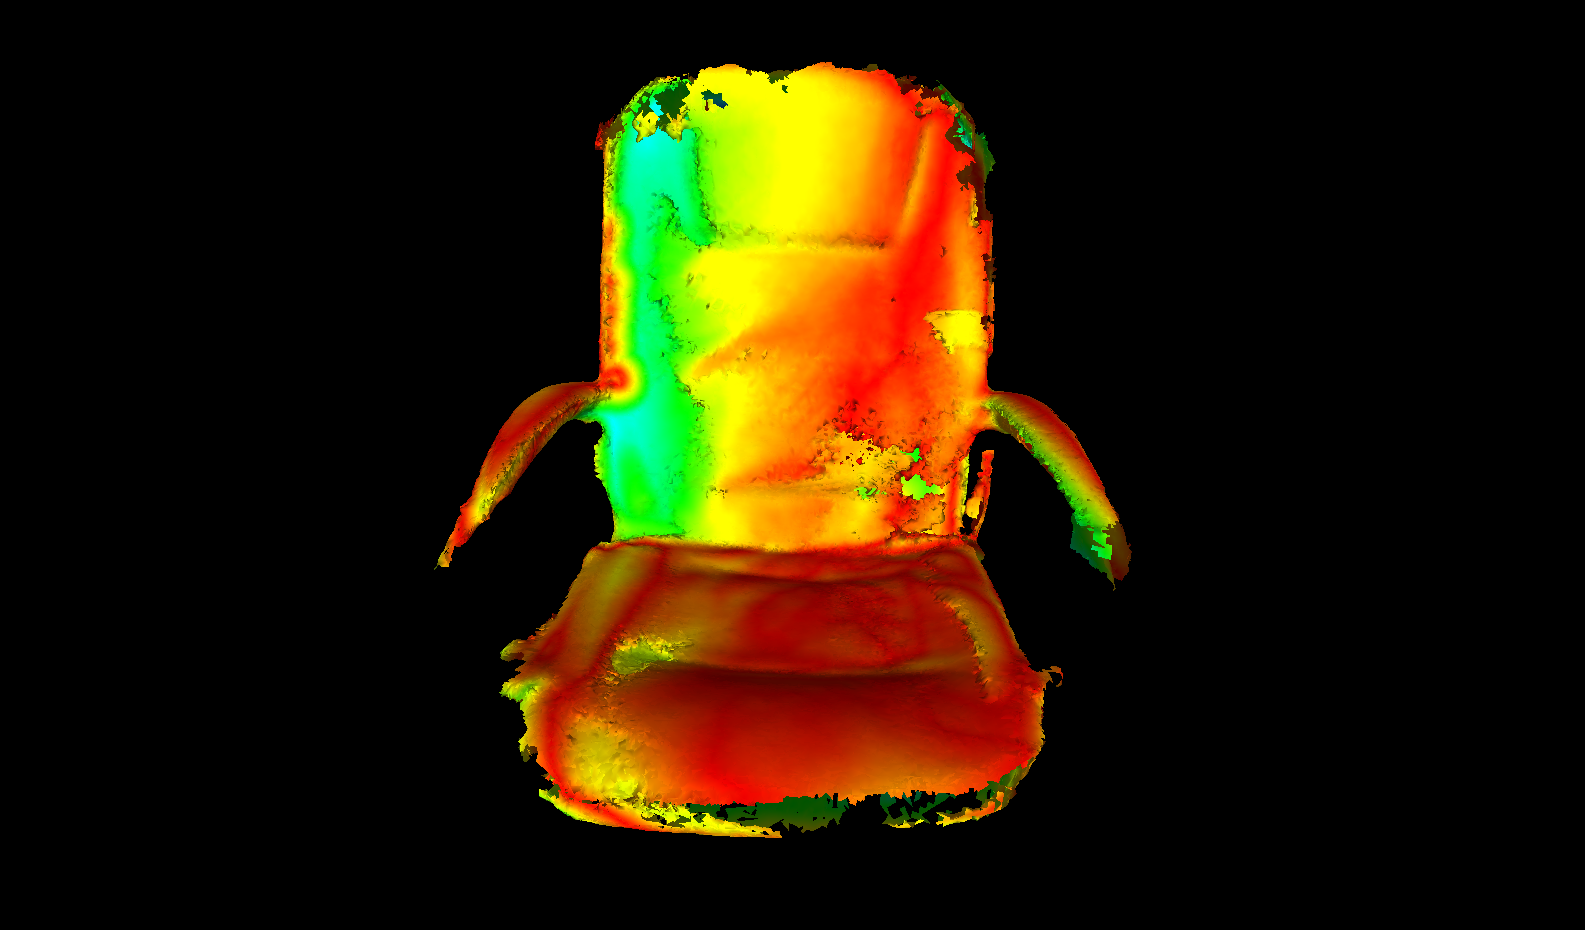
\includegraphics[width=.2\linewidth]{figures/object_recon/hauss/chair.png}&
      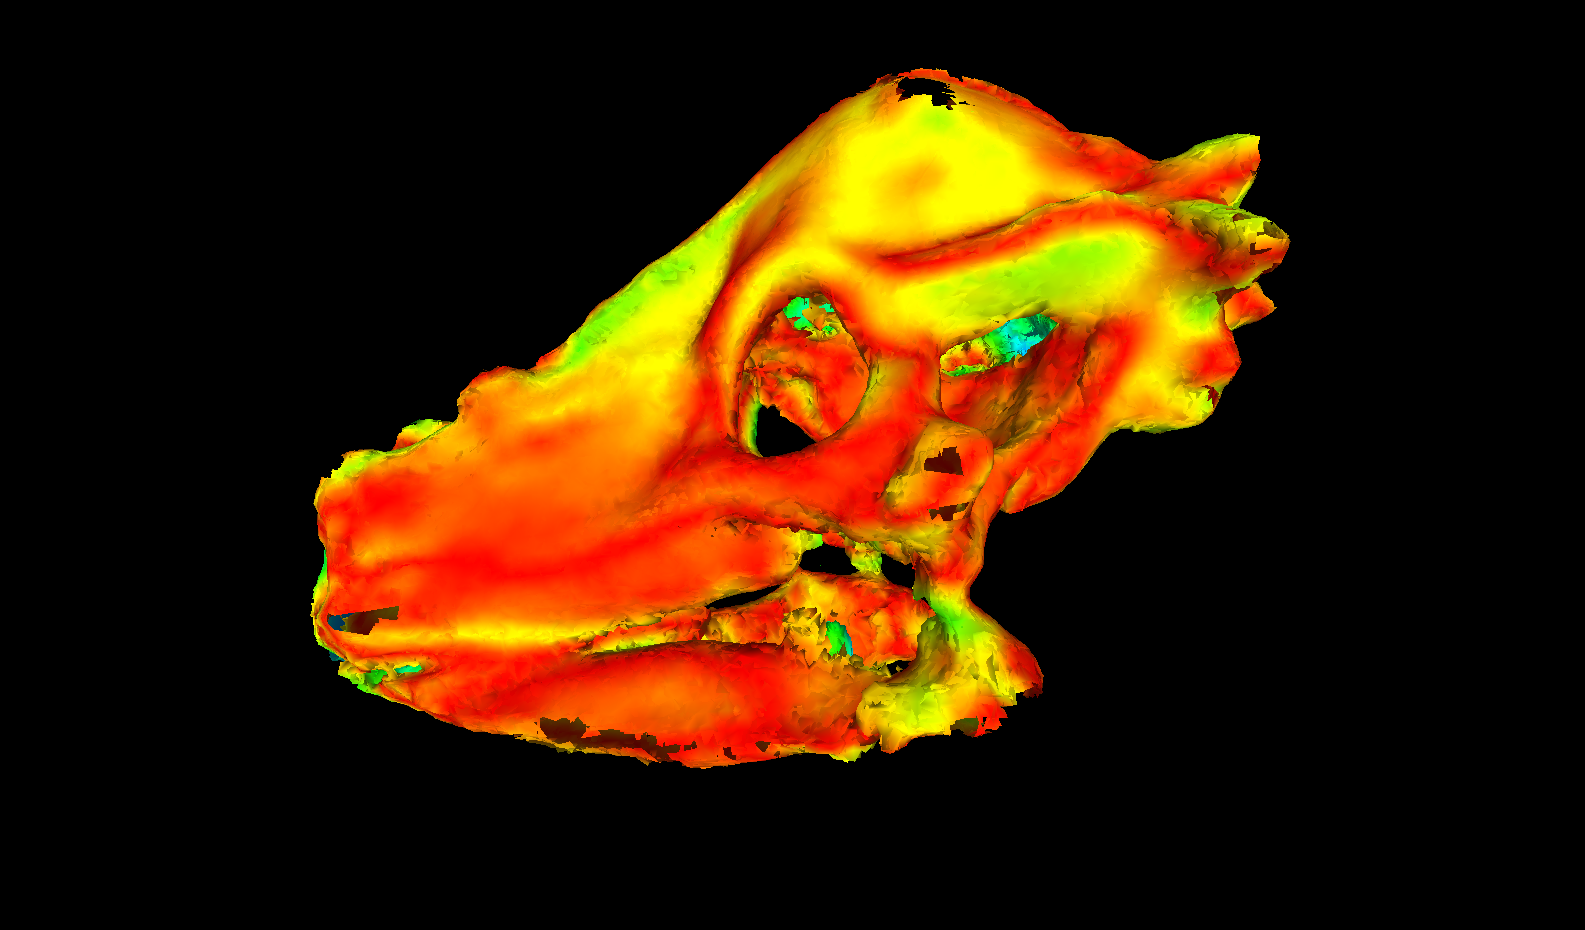
\includegraphics[width=.2\linewidth]{figures/object_recon/hauss/dino.png} \\
      (a) & (b) & (c) & (d) \\
    \end{tabular} \\
    \begin{tabular}{ccc}
      \textit{Max} & 
      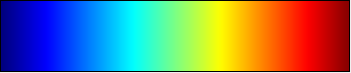
\includegraphics[width=.2\linewidth]{figures/object_recon/hauss/colour_range.png} & 
      \textit{Min} \\
      & (e) & \\
    \end{tabular}
  \end{tabular}
  \caption[Probabilistic Object Reconstruction Hausdorff Distance]
  {Renderings of the sequences evaluated in Table \ref{tbl:probobj_hauss} textured 
  on Hausdorff Distance (a, b, c, d). The minimum and maximum values given in Table 
  \ref{tbl:probobj_hauss} are mapped to the colour range of (e).}
\end{figure}

\section{Discussion}
\label{sec:probobj_discussion}
It is evident from Sections \ref{sec:sec:probobj_qualitative} and \ref{sec:probobj_quantitative} 
that the proposed approach is capable of densely reconstructing a range of rigid objects, providing 
closed and consistent object models, versus the state-of-the-art approach of \textit{Ren et al} 
\cite{Ren2013}, which failed to reconstruct any of the objects with nontrivial geometry that it 
was evaluated on. Additionally, the proposed approach shows an improvement over direct segmentation 
in image space of the object of interest in terms of pose estimation. When evaluating the output 
reconstructions of the proposed system versus those extracted from a standard \textit{KinectFusion} 
like pipeline (post reconstruction), the proposed system is capable of producing reconstructions that 
are geometrically similar.

The probabilistic formulation proposed in this work is intended to be easily generalised, such that 
it may be adapted for a range of use cases. For example, when utilising stereo sensors where a noise 
model may not be known a-priori, the framework allows for a suitable prior to be used. Additionally, 
the proposed approach is intentionally decoupled from the object segmentation model, allowing for 
ease of adaption for multiple object scenarios, or those where a continuous distribution over voxel 
labellings is required.